\documentclass[17pt, table, compress]{beamer}

%%%%%%%%%%%%  LATEX - BEAMERCLASS PRESENTATION DRAFT FOR ARVE %%%%%%%%%%%%%%%%%%%%
%
% We recommend to use the example page as a template for your presentation. A mini-
% mum working example for every frame is given by:
%
% \begin{frame}[t]{title}
% \vspace{0.7cm}
%	 Content
% \end{frame}
%
%%%%%%%%%%%%%%%%%%%%%%%%%%%%%%%%%%%%%%%%%%%%%%%%%%%%%%%%%%%%%%%%%%%%%%%%%%%%%%%%%%%%%


%%%%%%%%%%%%%%%%%%%%%%%   PLEASE DO NOT CHANGE THIS PART   %%%%%%%%%%%%%%%%%%%%%%%%%%
\useoutertheme{miniframes}
\useinnertheme{rectangles}
\usepackage[utf8x]{inputenc}
\usepackage[english]{babel}
\usepackage{xcolor}
\usepackage{listings}
\usepackage{amsmath}
\usepackage{amsfonts}
\usepackage{amssymb}
\usepackage{graphicx}
\usepackage{geometry}
\usepackage{helvet}
\usepackage[overlay, absolute]{textpos}
\usepackage[percent]{overpic}
\usepackage{setspace}
\renewcommand{\familydefault}{\sfdefault}
\usepackage{color}
\usepackage{framed}
\usepackage{cleveref}
\usepackage[fit,breakall]{truncate}
\usepackage[authoryear, round]{natbib}
\geometry{papersize={25.4cm,19.05cm}}
\setbeamertemplate{navigation symbols}{}
\setbeamertemplate{caption}{\insertcaption}
\definecolor{hereongreen}{RGB}{0, 145, 160}
\definecolor{hereonblue}{RGB}{0, 120, 210}
\definecolor{hereondarkblue}{RGB}{0, 70, 125}
\definecolor{hereondarkblueshaded}{RGB}{150, 180, 200}
\definecolor{hereonred}{RGB}{230, 0, 70}
\setbeamercolor{itemize item}{bg=hereondarkblue, fg=hereondarkblue}
\setbeamercolor{itemize subitem}{bg=black, fg=black}
\setbeamercolor{item}{bg=hereondarkblue, fg=hereondarkblue}
\setbeamertemplate{items}[circle]
\setbeamercolor{titlepalette}{fg=hereondarkblue}
\setbeamercolor{titlelike}{parent=titlepalette}
\setbeamercolor{block title}{fg=hereonblue}
\setbeamercolor{block title alerted}{fg=hereonred}
\setbeamerfont{block title}{series=\bfseries}
\setbeamerfont{frametitle}{size=\Large,series=\bfseries}

\newcommand{\tabitem}{~~\llap{\textcolor{hereondarkblue}{\Large \textbullet}}~~}

%%% BEAMER BUTTONS %%%
\setbeamertemplate{button}{\tikz
	\node[
	inner xsep=10pt,
	draw=structure!80,
	fill=hereongreen,
	rounded corners=4pt]  {\insertbuttontext};}

\usepackage{etoolbox}

\newcounter{NumSlidesCounter}

\makeatletter
\apptocmd{\beamer@@frametitle}{\write\@auxout{\string\@writefile{frm}{\string\frametitleentry{\the\c@framenumber}{#1}{#2}}}}{}{}
\newcommand*{\frametitleentry}[3]{\@namedef{frametitleshort#1}{#2}\@namedef{frametitle#1}{#3}}
\AtEndDocument{\if@filesw\newwrite\tf@frm\immediate\openout\tf@frm\jobname.frm\relax\fi}
\@input{\jobname.frm}
\newcommand*{\insertpreviousframetitle}[1][1]{\bgroup\advance\c@framenumber by -#1\relax\@nameuse{frametitleshort\the\c@framenumber}\egroup}
\newcommand*{\insertnextframetitle}[1][1]{\bgroup\advance\c@framenumber by #1\relax\@nameuse{frametitleshort\the\c@framenumber}\egroup}

\newcommand{\calcNumSlidesCounter}{%
	\setcounter{NumSlidesCounter}{\beamer@endpageofframe}%
	\addtocounter{NumSlidesCounter}{1}%
	\addtocounter{NumSlidesCounter}{-\beamer@startpageofframe}%
}

% increase footheight slighly to take care of continuation buttons
\patchcmd{\beamer@calculateheadfoot}{\advance\footheight by 4pt}{\advance\footheight by 20pt}{}{}

\makeatother

\newcommand{\continuationbuttons}{\slidebuttonsnum{\insertcontinuationcount}}

\newcommand{\slidebuttons}{\slidebuttonsnum{\overlaynumber}}

\newcommand{\slidebuttonsnum}[1]{%
	{
		\centering
		\calcNumSlidesCounter%
		\ifnum\theNumSlidesCounter>1
			\ifnum\theNumSlidesCounter>2
				\hyperlinkframestart{\beamerbutton{\Large $\ll$}}%
			\fi
			\hyperlinkslideprev{\beamerbutton{\Large $<$}}
			{\Large{#1/\theNumSlidesCounter}}
			\hyperlinkslidenext{\beamerbutton{\Large $>$}}
			\ifnum\theNumSlidesCounter>2
				\hyperlinkframeend{\beamerbutton{\Large $\gg$}}%
			\fi
		\fi
	}
}

\setbeamertemplate{footline}
{
	% do not increase the framenumber for frames with allowframebreak,
	% otherwise the button is not labeled correctly
	\ifnum\insertcontinuationcount>0 %
		\ifnum\insertpagenumber>\insertframestartpage
			\addtocounter{framenumber}{-1}
		\fi
		\hspace{0.05\linewidth}\continuationbuttons \\
	\fi
	\begin{columns}[c]
		\begin{column}{0.45\linewidth}
			\ifthenelse{\insertframenumber<3}{}{%
				\hyperlinkframeendprev{\beamerbutton{\large $\blacktriangleleft$  \,\truncate{0.8\linewidth}{\insertpreviousframetitle}}}
			}
		\end{column}
		\begin{column}{0.05\linewidth}
			\begin{tabular}{c}

				\setbeamertemplate{button}{\tikz
					\node[
					inner xsep=10pt,
					draw=structure!80,
					fill=hereondarkblue,
					rounded corners=4pt]  {\insertbuttontext};}

				\hyperlink{sec:home}{\beamerbutton{
\includegraphics[height=2em]{figures/home.png}}} \\
				
\includegraphics[height=0.8cm]{figures/CreativeCommons_Attribution_License.png}
			\end{tabular}
		\end{column}
		\begin{column}{0.45\linewidth}
		\hfill%
		\ifthenelse{\insertframenumber=\inserttotalframenumber}{}{%
			\hyperlinkframestartnext{\beamerbutton{\large\truncate{0.8\linewidth}{\insertnextframetitle}\, $\blacktriangleright$ }}
		}
		\end{column}
	\end{columns}
	\vspace{0.2em}
	\begin{footnotesize}
		\hspace{0.01\linewidth}
		\presentationsubtitle \, --
		\hyperlink{frm:author}{\presentationauthor} \, --
		\presentationdate
	\end{footnotesize}
	\vspace{0.2em}
}


%%% END BUTTONS %%%%

%%% FRAMETITLE %%%%

\setbeamertemplate{frametitle}
{
	\nointerlineskip
	\begin{beamercolorbox}[sep=0.3cm,wd=\paperwidth]{frametitle}
	\strut{\fontsize{28pt}{30pt}\selectfont \insertframetitle}\strut
	\hfill
	\raisebox{-6.0mm}{\hyperlink{sec:authors}{
\includegraphics[height=1.5em]{figures/hereon.png}}}
	\end{beamercolorbox}
}

%%% END FRAMETITLE %%%%

\makeatletter
\newcommand*{\overlaynumber}{\number\beamer@slideinframe}
\newcommand*{\numslides}{\number\beamer@minimum}
\makeatother

%%%%%%%%%%%%%%%%   HERE IS SOME SPACE FOR YOUR PERSONAL REAMBLES %%%%%%%%%%%%%%%%%%%%
\usepackage[loop]{animate}
\usepackage{setspace}
\usepackage{tikz}
\usepackage{wrapfig}  % To wrap text around a figure
\usetikzlibrary{arrows,shapes,tikzmark,fit,positioning,matrix,scopes,chains,overlay-beamer-styles, calc}
% tikzmark command, for shading over items
\newcommand{\mytikzmark}[1]{\tikz[overlay,remember picture] \node (#1) {};}
\newcommand{\mydottedline}{\color{blue}\makebox[0pt]{\textbullet}\hskip-0.5pt\vrule width 1pt\hspace{\labelsep}}
\usepackage{rotating}
\addtobeamertemplate{block begin}{\setlength\abovedisplayskip{0pt}}
% \setbeamerfont{itemize/enumerate subbody}{size=\normalsize} %to set the body size

\def\imagetop#1{\vtop{\null\hbox{#1}}}

%%% Presentation informations - FILL IN TITLE, SUBTITLE, etc. %%%
\newcommand{\presentationtitle}{Model Data Explorer}
\newcommand{\presentationsubtitle}{ESM Data Exploration with the Model Data Explorer}
\newcommand{\presentationdate}{April 29th, 2023}
\newcommand{\location}{EGU, Vienna, Austria}
\newcommand{\presentationauthor}{Philipp S. Sommer}
\newcommand{\authoremail}{philipp.sommer@hereon.de}

%\AtBeginSubsection[]{
%	\begin{frame}
%		\vfill
%		\centering
%		\begin{beamercolorbox}[sep=8pt,center,shadow=true,rounded=true]{title}
%			\usebeamerfont{title}\insertsectionhead \\ \insertsubsectionhead\par%
%		\end{beamercolorbox}
%		\vfill
%	\end{frame}
%}

%%%%%%%%%%%%%%%%%%%%%%%

%%%%%%%% Listings style %%%%%%%%
\definecolor{DarkGreen}{rgb}{0.0,0.4,0.0} % Comment color
\definecolor{highlight}{RGB}{255,251,204} % Code highlight color

\lstdefinestyle{Style1}{ % Define a style for your code snippet, multiple definitions can be made if, for example, you wish to insert multiple code snippets using different programming languages into one document
	language=bash, % Detects keywords, comments, strings, functions, etc for the language specified
	backgroundcolor=\color[gray]{0.9}, % Set the background color for the snippet - useful for highlighting
	basicstyle=\small\ttfamily, % The default font size and style of the code
	breakatwhitespace=false, % If true, only allows line breaks at white space
	breaklines=true, % Automatic line breaking (prevents code from protruding outside the box)
	captionpos=b, % Sets the caption position: b for bottom; t for top
	commentstyle=\color{DarkGreen}, % Style of comments within the code - dark green courier font
	deletekeywords={}, % If you want to delete any keywords from the current language separate them by commas
	%escapeinside={\%}, % This allows you to escape to LaTeX using the character in the bracket
	firstnumber=1, % Line numbers begin at line 1
	frame=single, % Frame around the code box, value can be: none, leftline, topline, bottomline, lines, single, shadowbox
	frameround=tttt, % Rounds the corners of the frame for the top left, top right, bottom left and bottom right positions
%	keywordstyle=blue, % Functions are bold and blue
	morekeywords={}, % Add any functions no included by default here separated by commas
	numbers=left, % Location of line numbers, can take the values of: none, left, right
	numbersep=10pt, % Distance of line numbers from the code box
	numberstyle=\tiny\color{gray}, % Style used for line numbers
	rulecolor=\color{black}, % Frame border color
	showstringspaces=false, % Don't put marks in string spaces
	showtabs=false, % Display tabs in the code as lines
	stepnumber=5, % The step distance between line numbers, i.e. how often will lines be numbered
	stringstyle=\color{purple}, % Strings are purple
	tabsize=4, % Number of spaces per tab in the code
}
\lstset{style=Style1}
% Create a command to cleanly insert a snippet with the style above anywhere in the document
\newcommand{\insertcode}[2]{\begin{itemize}\item[]\lstinputlisting[caption=#2,label=#1,style=Style1]{#1}\end{itemize}} % The first argument is the script location/filename and the second is a caption for the

%%%%%%%% END listings style %%%%%%%%%%5

\title{\presentationtitle}
\subtitle{\presentationsubtitle}
\date{\presentationdate}
\author{\presentationauthor}

\hypersetup{
    colorlinks,
	linkcolor={gray!80!black},
	citecolor={black},
	urlcolor={gray!80!black},
	pdfauthor=\presentationauthor,
	pdfsubject={Model Data Explorer},
	pdftitle=\presentationtitle - \presentationsubtitle,
	pdfkeywords={django, model data, FAIR, Earth System Models, Climate Models},
	pdfstartpage=1
}

% !TeX root = psyplot-presentation.tex

%%%%% EXAMPLES FORMATTING %%%%%%5%%%%
\usepackage{adjustbox} % Used to constrain images to a maximum size 
\usepackage{textcomp} % defines textquotesingle
\usepackage{upquote} % Upright quotes for verbatim code
\usepackage{fancyvrb} % verbatim replacement that allows latex

    % commands and environments needed by pandoc snippets
% extracted from the output of `pandoc -s`
\providecommand{\tightlist}{%
	\setlength{\itemsep}{0pt}\setlength{\parskip}{0pt}}
\DefineVerbatimEnvironment{Highlighting}{Verbatim}{commandchars=\\\{\}}
% Add ',fontsize=\small' for more characters per line
\newenvironment{Shaded}{}{}
\newcommand{\KeywordTok}[1]{\textcolor[rgb]{0.00,0.44,0.13}{\textbf{{#1}}}}
\newcommand{\DataTypeTok}[1]{\textcolor[rgb]{0.56,0.13,0.00}{{#1}}}
\newcommand{\DecValTok}[1]{\textcolor[rgb]{0.25,0.63,0.44}{{#1}}}
\newcommand{\BaseNTok}[1]{\textcolor[rgb]{0.25,0.63,0.44}{{#1}}}
\newcommand{\FloatTok}[1]{\textcolor[rgb]{0.25,0.63,0.44}{{#1}}}
\newcommand{\CharTok}[1]{\textcolor[rgb]{0.25,0.44,0.63}{{#1}}}
\newcommand{\StringTok}[1]{\textcolor[rgb]{0.25,0.44,0.63}{{#1}}}
\newcommand{\CommentTok}[1]{\textcolor[rgb]{0.38,0.63,0.69}{\textit{{#1}}}}
\newcommand{\OtherTok}[1]{\textcolor[rgb]{0.00,0.44,0.13}{{#1}}}
\newcommand{\AlertTok}[1]{\textcolor[rgb]{1.00,0.00,0.00}{\textbf{{#1}}}}
\newcommand{\FunctionTok}[1]{\textcolor[rgb]{0.02,0.16,0.49}{{#1}}}
\newcommand{\RegionMarkerTok}[1]{{#1}}
\newcommand{\ErrorTok}[1]{\textcolor[rgb]{1.00,0.00,0.00}{\textbf{{#1}}}}
\newcommand{\NormalTok}[1]{{#1}}

% Additional commands for more recent versions of Pandoc
\newcommand{\ConstantTok}[1]{\textcolor[rgb]{0.53,0.00,0.00}{{#1}}}
\newcommand{\SpecialCharTok}[1]{\textcolor[rgb]{0.25,0.44,0.63}{{#1}}}
\newcommand{\VerbatimStringTok}[1]{\textcolor[rgb]{0.25,0.44,0.63}{{#1}}}
\newcommand{\SpecialStringTok}[1]{\textcolor[rgb]{0.73,0.40,0.53}{{#1}}}
\newcommand{\ImportTok}[1]{{#1}}
\newcommand{\DocumentationTok}[1]{\textcolor[rgb]{0.73,0.13,0.13}{\textit{{#1}}}}
\newcommand{\AnnotationTok}[1]{\textcolor[rgb]{0.38,0.63,0.69}{\textbf{\textit{{#1}}}}}
\newcommand{\CommentVarTok}[1]{\textcolor[rgb]{0.38,0.63,0.69}{\textbf{\textit{{#1}}}}}
\newcommand{\VariableTok}[1]{\textcolor[rgb]{0.10,0.09,0.49}{{#1}}}
\newcommand{\ControlFlowTok}[1]{\textcolor[rgb]{0.00,0.44,0.13}{\textbf{{#1}}}}
\newcommand{\OperatorTok}[1]{\textcolor[rgb]{0.40,0.40,0.40}{{#1}}}
\newcommand{\BuiltInTok}[1]{{#1}}
\newcommand{\ExtensionTok}[1]{{#1}}
\newcommand{\PreprocessorTok}[1]{\textcolor[rgb]{0.74,0.48,0.00}{{#1}}}
\newcommand{\AttributeTok}[1]{\textcolor[rgb]{0.49,0.56,0.16}{{#1}}}
\newcommand{\InformationTok}[1]{\textcolor[rgb]{0.38,0.63,0.69}{\textbf{\textit{{#1}}}}}
\newcommand{\WarningTok}[1]{\textcolor[rgb]{0.38,0.63,0.69}{\textbf{\textit{{#1}}}}}

% ANSI colors
\definecolor{ansi-black}{HTML}{3E424D}
\definecolor{ansi-black-intense}{HTML}{282C36}
\definecolor{ansi-red}{HTML}{E75C58}
\definecolor{ansi-red-intense}{HTML}{B22B31}
\definecolor{ansi-green}{HTML}{00A250}
\definecolor{ansi-green-intense}{HTML}{007427}
\definecolor{ansi-yellow}{HTML}{DDB62B}
\definecolor{ansi-yellow-intense}{HTML}{B27D12}
\definecolor{ansi-blue}{HTML}{208FFB}
\definecolor{ansi-blue-intense}{HTML}{0065CA}
\definecolor{ansi-magenta}{HTML}{D160C4}
\definecolor{ansi-magenta-intense}{HTML}{A03196}
\definecolor{ansi-cyan}{HTML}{60C6C8}
\definecolor{ansi-cyan-intense}{HTML}{258F8F}
\definecolor{ansi-white}{HTML}{C5C1B4}
\definecolor{ansi-white-intense}{HTML}{A1A6B2}

% Pygments definitions

\makeatletter
\def\PY@reset{\let\PY@it=\relax \let\PY@bf=\relax%
	\let\PY@ul=\relax \let\PY@tc=\relax%
	\let\PY@bc=\relax \let\PY@ff=\relax}
\def\PY@tok#1{\csname PY@tok@#1\endcsname}
\def\PY@toks#1+{\ifx\relax#1\empty\else%
	\PY@tok{#1}\expandafter\PY@toks\fi}
\def\PY@do#1{\PY@bc{\PY@tc{\PY@ul{%
				\PY@it{\PY@bf{\PY@ff{#1}}}}}}}
\def\PY#1#2{\PY@reset\PY@toks#1+\relax+\PY@do{#2}}

\expandafter\def\csname PY@tok@w\endcsname{\def\PY@tc##1{\textcolor[rgb]{0.73,0.73,0.73}{##1}}}
\expandafter\def\csname PY@tok@c\endcsname{\let\PY@it=\textit\def\PY@tc##1{\textcolor[rgb]{0.25,0.50,0.50}{##1}}}
\expandafter\def\csname PY@tok@cp\endcsname{\def\PY@tc##1{\textcolor[rgb]{0.74,0.48,0.00}{##1}}}
\expandafter\def\csname PY@tok@k\endcsname{\let\PY@bf=\textbf\def\PY@tc##1{\textcolor[rgb]{0.00,0.50,0.00}{##1}}}
\expandafter\def\csname PY@tok@kp\endcsname{\def\PY@tc##1{\textcolor[rgb]{0.00,0.50,0.00}{##1}}}
\expandafter\def\csname PY@tok@kt\endcsname{\def\PY@tc##1{\textcolor[rgb]{0.69,0.00,0.25}{##1}}}
\expandafter\def\csname PY@tok@o\endcsname{\def\PY@tc##1{\textcolor[rgb]{0.40,0.40,0.40}{##1}}}
\expandafter\def\csname PY@tok@ow\endcsname{\let\PY@bf=\textbf\def\PY@tc##1{\textcolor[rgb]{0.67,0.13,1.00}{##1}}}
\expandafter\def\csname PY@tok@nb\endcsname{\def\PY@tc##1{\textcolor[rgb]{0.00,0.50,0.00}{##1}}}
\expandafter\def\csname PY@tok@nf\endcsname{\def\PY@tc##1{\textcolor[rgb]{0.00,0.00,1.00}{##1}}}
\expandafter\def\csname PY@tok@nc\endcsname{\let\PY@bf=\textbf\def\PY@tc##1{\textcolor[rgb]{0.00,0.00,1.00}{##1}}}
\expandafter\def\csname PY@tok@nn\endcsname{\let\PY@bf=\textbf\def\PY@tc##1{\textcolor[rgb]{0.00,0.00,1.00}{##1}}}
\expandafter\def\csname PY@tok@ne\endcsname{\let\PY@bf=\textbf\def\PY@tc##1{\textcolor[rgb]{0.82,0.25,0.23}{##1}}}
\expandafter\def\csname PY@tok@nv\endcsname{\def\PY@tc##1{\textcolor[rgb]{0.10,0.09,0.49}{##1}}}
\expandafter\def\csname PY@tok@no\endcsname{\def\PY@tc##1{\textcolor[rgb]{0.53,0.00,0.00}{##1}}}
\expandafter\def\csname PY@tok@nl\endcsname{\def\PY@tc##1{\textcolor[rgb]{0.63,0.63,0.00}{##1}}}
\expandafter\def\csname PY@tok@ni\endcsname{\let\PY@bf=\textbf\def\PY@tc##1{\textcolor[rgb]{0.60,0.60,0.60}{##1}}}
\expandafter\def\csname PY@tok@na\endcsname{\def\PY@tc##1{\textcolor[rgb]{0.49,0.56,0.16}{##1}}}
\expandafter\def\csname PY@tok@nt\endcsname{\let\PY@bf=\textbf\def\PY@tc##1{\textcolor[rgb]{0.00,0.50,0.00}{##1}}}
\expandafter\def\csname PY@tok@nd\endcsname{\def\PY@tc##1{\textcolor[rgb]{0.67,0.13,1.00}{##1}}}
\expandafter\def\csname PY@tok@s\endcsname{\def\PY@tc##1{\textcolor[rgb]{0.73,0.13,0.13}{##1}}}
\expandafter\def\csname PY@tok@sd\endcsname{\let\PY@it=\textit\def\PY@tc##1{\textcolor[rgb]{0.73,0.13,0.13}{##1}}}
\expandafter\def\csname PY@tok@si\endcsname{\let\PY@bf=\textbf\def\PY@tc##1{\textcolor[rgb]{0.73,0.40,0.53}{##1}}}
\expandafter\def\csname PY@tok@se\endcsname{\let\PY@bf=\textbf\def\PY@tc##1{\textcolor[rgb]{0.73,0.40,0.13}{##1}}}
\expandafter\def\csname PY@tok@sr\endcsname{\def\PY@tc##1{\textcolor[rgb]{0.73,0.40,0.53}{##1}}}
\expandafter\def\csname PY@tok@ss\endcsname{\def\PY@tc##1{\textcolor[rgb]{0.10,0.09,0.49}{##1}}}
\expandafter\def\csname PY@tok@sx\endcsname{\def\PY@tc##1{\textcolor[rgb]{0.00,0.50,0.00}{##1}}}
\expandafter\def\csname PY@tok@m\endcsname{\def\PY@tc##1{\textcolor[rgb]{0.40,0.40,0.40}{##1}}}
\expandafter\def\csname PY@tok@gh\endcsname{\let\PY@bf=\textbf\def\PY@tc##1{\textcolor[rgb]{0.00,0.00,0.50}{##1}}}
\expandafter\def\csname PY@tok@gu\endcsname{\let\PY@bf=\textbf\def\PY@tc##1{\textcolor[rgb]{0.50,0.00,0.50}{##1}}}
\expandafter\def\csname PY@tok@gd\endcsname{\def\PY@tc##1{\textcolor[rgb]{0.63,0.00,0.00}{##1}}}
\expandafter\def\csname PY@tok@gi\endcsname{\def\PY@tc##1{\textcolor[rgb]{0.00,0.63,0.00}{##1}}}
\expandafter\def\csname PY@tok@gr\endcsname{\def\PY@tc##1{\textcolor[rgb]{1.00,0.00,0.00}{##1}}}
\expandafter\def\csname PY@tok@ge\endcsname{\let\PY@it=\textit}
\expandafter\def\csname PY@tok@gs\endcsname{\let\PY@bf=\textbf}
\expandafter\def\csname PY@tok@gp\endcsname{\let\PY@bf=\textbf\def\PY@tc##1{\textcolor[rgb]{0.00,0.00,0.50}{##1}}}
\expandafter\def\csname PY@tok@go\endcsname{\def\PY@tc##1{\textcolor[rgb]{0.53,0.53,0.53}{##1}}}
\expandafter\def\csname PY@tok@gt\endcsname{\def\PY@tc##1{\textcolor[rgb]{0.00,0.27,0.87}{##1}}}
\expandafter\def\csname PY@tok@err\endcsname{\def\PY@bc##1{\setlength{\fboxsep}{0pt}\fcolorbox[rgb]{1.00,0.00,0.00}{1,1,1}{\strut ##1}}}
\expandafter\def\csname PY@tok@kc\endcsname{\let\PY@bf=\textbf\def\PY@tc##1{\textcolor[rgb]{0.00,0.50,0.00}{##1}}}
\expandafter\def\csname PY@tok@kd\endcsname{\let\PY@bf=\textbf\def\PY@tc##1{\textcolor[rgb]{0.00,0.50,0.00}{##1}}}
\expandafter\def\csname PY@tok@kn\endcsname{\let\PY@bf=\textbf\def\PY@tc##1{\textcolor[rgb]{0.00,0.50,0.00}{##1}}}
\expandafter\def\csname PY@tok@kr\endcsname{\let\PY@bf=\textbf\def\PY@tc##1{\textcolor[rgb]{0.00,0.50,0.00}{##1}}}
\expandafter\def\csname PY@tok@bp\endcsname{\def\PY@tc##1{\textcolor[rgb]{0.00,0.50,0.00}{##1}}}
\expandafter\def\csname PY@tok@fm\endcsname{\def\PY@tc##1{\textcolor[rgb]{0.00,0.00,1.00}{##1}}}
\expandafter\def\csname PY@tok@vc\endcsname{\def\PY@tc##1{\textcolor[rgb]{0.10,0.09,0.49}{##1}}}
\expandafter\def\csname PY@tok@vg\endcsname{\def\PY@tc##1{\textcolor[rgb]{0.10,0.09,0.49}{##1}}}
\expandafter\def\csname PY@tok@vi\endcsname{\def\PY@tc##1{\textcolor[rgb]{0.10,0.09,0.49}{##1}}}
\expandafter\def\csname PY@tok@vm\endcsname{\def\PY@tc##1{\textcolor[rgb]{0.10,0.09,0.49}{##1}}}
\expandafter\def\csname PY@tok@sa\endcsname{\def\PY@tc##1{\textcolor[rgb]{0.73,0.13,0.13}{##1}}}
\expandafter\def\csname PY@tok@sb\endcsname{\def\PY@tc##1{\textcolor[rgb]{0.73,0.13,0.13}{##1}}}
\expandafter\def\csname PY@tok@sc\endcsname{\def\PY@tc##1{\textcolor[rgb]{0.73,0.13,0.13}{##1}}}
\expandafter\def\csname PY@tok@dl\endcsname{\def\PY@tc##1{\textcolor[rgb]{0.73,0.13,0.13}{##1}}}
\expandafter\def\csname PY@tok@s2\endcsname{\def\PY@tc##1{\textcolor[rgb]{0.73,0.13,0.13}{##1}}}
\expandafter\def\csname PY@tok@sh\endcsname{\def\PY@tc##1{\textcolor[rgb]{0.73,0.13,0.13}{##1}}}
\expandafter\def\csname PY@tok@s1\endcsname{\def\PY@tc##1{\textcolor[rgb]{0.73,0.13,0.13}{##1}}}
\expandafter\def\csname PY@tok@mb\endcsname{\def\PY@tc##1{\textcolor[rgb]{0.40,0.40,0.40}{##1}}}
\expandafter\def\csname PY@tok@mf\endcsname{\def\PY@tc##1{\textcolor[rgb]{0.40,0.40,0.40}{##1}}}
\expandafter\def\csname PY@tok@mh\endcsname{\def\PY@tc##1{\textcolor[rgb]{0.40,0.40,0.40}{##1}}}
\expandafter\def\csname PY@tok@mi\endcsname{\def\PY@tc##1{\textcolor[rgb]{0.40,0.40,0.40}{##1}}}
\expandafter\def\csname PY@tok@il\endcsname{\def\PY@tc##1{\textcolor[rgb]{0.40,0.40,0.40}{##1}}}
\expandafter\def\csname PY@tok@mo\endcsname{\def\PY@tc##1{\textcolor[rgb]{0.40,0.40,0.40}{##1}}}
\expandafter\def\csname PY@tok@ch\endcsname{\let\PY@it=\textit\def\PY@tc##1{\textcolor[rgb]{0.25,0.50,0.50}{##1}}}
\expandafter\def\csname PY@tok@cm\endcsname{\let\PY@it=\textit\def\PY@tc##1{\textcolor[rgb]{0.25,0.50,0.50}{##1}}}
\expandafter\def\csname PY@tok@cpf\endcsname{\let\PY@it=\textit\def\PY@tc##1{\textcolor[rgb]{0.25,0.50,0.50}{##1}}}
\expandafter\def\csname PY@tok@c1\endcsname{\let\PY@it=\textit\def\PY@tc##1{\textcolor[rgb]{0.25,0.50,0.50}{##1}}}
\expandafter\def\csname PY@tok@cs\endcsname{\let\PY@it=\textit\def\PY@tc##1{\textcolor[rgb]{0.25,0.50,0.50}{##1}}}

\def\PYZbs{\char`\\}
\def\PYZus{\char`\_}
\def\PYZob{\char`\{}
\def\PYZcb{\char`\}}
\def\PYZca{\char`\^}
\def\PYZam{\char`\&}
\def\PYZlt{\char`\<}
\def\PYZgt{\char`\>}
\def\PYZsh{\char`\#}
\def\PYZpc{\char`\%}
\def\PYZdl{\char`\$}
\def\PYZhy{\char`\-}
\def\PYZsq{\char`\'}
\def\PYZdq{\char`\"}
\def\PYZti{\char`\~}
% for compatibility with earlier versions
\def\PYZat{@}
\def\PYZlb{[}
\def\PYZrb{]}
\makeatother


% Exact colors from NB
\definecolor{incolor}{rgb}{0.0, 0.0, 0.5}
\definecolor{outcolor}{rgb}{0.545, 0.0, 0.0}

\newcounter{continuationFirstSlide}
\setcounter{continuationFirstSlide}{1}
%%%%% END EXAMPLES FORMATTING %%%%%%%%

%%%%%%%%%%%%%%%%%%%   BEGIN OF THE MAIN PART OF THE DOCUMENT %%%%%%%%%%%%%%%%%%%%%%%%

%\includeonly{content/example_mapplotters}

\begin{document}
% For every picture that defines or uses external nodes, you'll have to
% apply the 'remember picture' style. To avoid some typing, we'll apply
% the style to all pictures.
\tikzstyle{every picture}+=[remember picture]

%%%%%%%%%%%%%%%%%%%%%% !! YOUR CONTENT BEGINS HERE !! %%%%%%%%%%%%%%%%%%%%%%%%%%%%%%%

%
%Includes
%
% !TeX root = ../mde-presentation.tex

\section{Home} \label{sec:home}
%%%%%%%%%%%%%%%%   HOME PAGE   %%%%%%%%%%%%%%%%%%

\begin{frame}[t, plain]{}

	\setbeamertemplate{button}{\tikz
	\node[
	inner xsep=20pt,
	inner ysep=10pt,
	minimum height=5em,
	draw=structure!80,
	fill=hereongreen,
	rounded corners=4pt]  {\insertbuttontext};}

	% title
	\begin{textblock*}{\linewidth}(0.05\linewidth, 0.05\textheight)
		\centering
		{\Large{Modern Earth system science visualization and exploration techniques}} \\ \vspace{1em}
		\presentationsubtitle \\
		\vspace{1em}
		ESSI4.1 | \location \, | \presentationdate

		\begin{columns}
			\begin{column}{0.5\linewidth}
				\begin{block}{\center Talk}
					\centering
					\vspace{1em}
					\hyperlink{sec:session-intro}{\beamerbutton{\large Session Intro}} \\
					\vspace{1em}
					\hyperlink{sec:madness}{\beamerbutton{\large 2-Minute Madness}}
				\end{block}
			\end{column}
			\begin{column}{0.5\linewidth}
				\begin{block}{\center General}
					\centering
					\vspace{1em}
					\begin{tabular}{ll}
						\hyperlink{sec:authors}{\beamerbutton{\large Author}} & \hyperlink{sec:funding}{\beamerbutton{\large Funding}} \\
					\end{tabular} \\
					\vspace{1em}
					\hyperlink{sec:abstract}{\beamerbutton{\large Abstract}}
				\end{block}
			\end{column}
		\end{columns}

		\begin{block}{\center Implementation}
			\begin{center}
				\hspace{2.5em}
				\hyperlink{sec:core}{\beamerbutton{\large Core}} \quad
				\hyperlink{sec:plugins}{\beamerbutton{\large Plugins}} \quad
				\hyperlink{sec:federation}{\beamerbutton{\large Federation}} \\

				\vspace{1em}

				\hyperlink{sec:maintenance}{\beamerbutton{\large Maintenance}} \quad
				\hyperlink{sec:resources}{\beamerbutton{\large Resources}}
			\end{center}
		\end{block}
	\end{textblock*}

	\begin{textblock*}{0.4\textwidth}(0.05\textwidth,0.94\textheight)
		\href{https://github.com/Chilipp/mde-presentation-egu2023}{
			
\includegraphics[width=4cm]{figures/qrcode-presentation.png}
		} \\
		\href{https://doi.org/10.5194/egusphere-egu23-3624}{
			
\includegraphics[width=\textwidth]{figures/doi.pdf}
		}
	\end{textblock*}

	\begin{textblock*}{6cm}(0.8\textwidth,1.05\textheight)
		\raggedleft
		\hyperlink{frm:map}{
\includegraphics[width=6cm]{figures/hereon.png}} \\
		
\includegraphics[height=0.8cm]{figures/CreativeCommons_Attribution_License.png}
	\end{textblock*}

\end{frame}

\section{Help} \label{sec:help}

\begin{frame}
	\frametitle[Help]{How to navigate}
	This presentation has been prepared for a PICO presentation at the EGU 2023 in Vienna, Austria. To facilitate the navigation, a lot of hyperlinks are used. Almost every item in this presentation is clickable:
	\begin{itemize}
		\item click \beamerbutton{buttons like this} to be linked to other connected frames
		\item click the navigation bar above with the sections, \hyperlink{sec:home}{Home}, \hyperlink{sec:help}{Help}, etc. (including the dots) to navigate in the presentation
		\item click on navigation buttons like this \slidebuttons to show you more of the current frame. \only<2>{\textcolor{red}{For example this text.}}
		\item click on many of the images to get more information or a close-up
		\item click the \hyperlink{sec:home}{\beamerbutton{
\includegraphics[height=0.8cm]{figures/home.png}}} icon to go back to the menu
		\item click the buttons at the lower left and lower right that bring you to the next slide
	\end{itemize}
\end{frame}
% !TeX root = ../mde-presentation.tex

\section{Session Introduction} \label{sec:session-intro}

\begin{frame}
	\frametitle[Session title page]{}
	\begin{center}
		{\color{black}
			\textbf{
				\fontsize{36pt}{38pt}\selectfont Modern Earth system science visualization and exploration techniques\\
				\vspace{1.5cm}}}
		\textbf{
			\fontsize{26pt}{28pt}\selectfont The balancing act between complex information, broad functionality and simple illustration \\
		}
		\vspace{1em}
		{\fontsize{18pt}{20pt}\selectfont
            ESSI4.1 | \location \, | \presentationdate \\
			\vspace{1em}
			Conveners: \\
            Tobias Kerzenmacher, Christof Lorenz, Ugur Cayoglu, \textbf{Philipp S. Sommer}}

	\end{center}

    \begin{textblock*}{\textwidth}(0.1\textwidth,0.95\textheight)
        \begin{tabular}{p{0.3\textwidth}p{0.3\textwidth}p{0.3\textwidth}}
            \href{https://kit.edu}{
\includegraphics[width=5cm]{figures/kit.pdf}} &
            \href{https://datahub.erde-und-umwelt.de}{
\includegraphics[width=5cm]{figures/datahub.png}} &
            \hyperlink{frm:map}{
\includegraphics[width=5cm]{figures/hereon.png}}
        \end{tabular}
    \end{textblock*}
\end{frame}

\begin{frame}{Challenges and opportunities}
    \begin{columns}[T]
        \begin{column}{0.45\linewidth}
            Earth system science data are getting increasingly important
            \begin{itemize}
                \item as decision support for stakeholders
                \item for other end users far beyond the scientific domains
                \item within project collaborations
                \item Institutes, Groups and projects are reviewed with respect
                    to the data products they publish
            \end{itemize}
        \end{column}
        \begin{column}{0.45\linewidth}
            But higher temporal and spatial resolutions of modeling and
            remote sensing approaches lead to ever-increasing data
            complexity and volumes

            \vspace{1em}

            \begin{alertblock}<2->{We want to prevent}
                \begin{itemize}
                    \item data that cannot be found
                    \item outdated and insecure software
                    \item always reinventing the wheel
                \end{itemize}
            \end{alertblock}

        \end{column}
    \end{columns}

    \begin{textblock*}{\textwidth}(0.05\linewidth, 1.07\textheight)
		\slidebuttons
	\end{textblock*}

\end{frame}

\begin{frame}{Data standards}
    Making data available can push the use of data standards that improve data
    findability, accessibility, interoperability and reusability (FAIR).

    \vspace{1em}

    \begin{columns}[T]
        \begin{column}<2->{0.6\textwidth}
            \begin{block}{Tool tips to improve data management}
                \begin{itemize}
                    \item use OGC standards for visualization
                    \item do not only visualize, provide download as well
                    \item correctly cite the data and publications you are showing
                    \item ask supplied data to fulfill certain metadata standards
                    \item provide instructions (e.g. in form of Standard Operating Procedures) on how to get different data into your software
                \end{itemize}
            \end{block}
        \end{column}
        \begin{column}{0.3\textwidth}
            
\includegraphics[width=\textwidth]{figures/FAIR_data_principles.jpg}
        \end{column}
    \end{columns}

    \begin{textblock*}{\textwidth}(0.05\linewidth, 1.07\textheight)
		\slidebuttons
	\end{textblock*}

\end{frame}

\begin{frame}{Research Software Recommendations}

    \begin{textblock*}{0.35\linewidth}(0.7\linewidth, 0.23\textheight)
        \slidebuttons
    \end{textblock*}

    \begin{columns}[t]
        \begin{column}{0.5\textwidth}
            \begin{block}{Tips for improving persistence}
                \begin{itemize}
                    \item make your software modular
                    \item invest time in the conceptualization of a software
                        framework
                    \item make it open-source
                    \item make it available in an open gitlab or on github
                    \item make your software installable in different infrastructures
                    \item package your software
                    \item version your software
                    \item containerize your software deployment-ready
                    \item provide login via eduGAIN or other AAI
                \end{itemize}
            \end{block}
        \end{column}
        \begin{column}{0.5\textwidth}
            \begin{block}<2->{Tips for implementing tests}
                \begin{itemize}
                    \item invest time in unit tests
                    \item invest time in stakeholder tests
                    \item automate your documentation
                    \item use continuous integration for testing your software
                \end{itemize}
            \end{block}
            \begin{block}<3->{Tips for documentation}
                \begin{itemize}
                    \item invest time in API documentation
                    \item describe your framework
                    \item provide detailed installation instructions
                \end{itemize}
            \end{block}
        \end{column}
    \end{columns}

\end{frame}

\begin{frame}[t]{Our session}
    A diverse set of tools that make Earth System Science Data available on the
    web

    \vspace{1em}

    \begin{itemize}
        \item Generic data exploration frameworks
        \item Personalized data exploration frameworks driven by a specific
            scientific use-case
        \item Transfer- and outreach-driven exploration frameworks
    \end{itemize}

    \vspace{1em}

    \begin{block}{Our hope}
        Establish a transdisciplinary community of scientists,
        software-developers and other experts in the field of data
        visualization in order to exchange and to give a state-of-the-art
        overview of tools, interfaces and best-practices.
    \end{block}
\end{frame}

% !TeX root = ../mde-presentation.tex

\section{2-Minute Madness} \label{sec:madness}
%%%%%%%%%%%%%%%%   TITLE PAGE   %%%%%%%%%%%%%%%%%%
\subsection*{Title page}  % to show it in the title bar

\begin{frame}
	\frametitle[MDE title page]{}
	\vspace{2.0cm}
	\begin{center}
		{\color{black}
			\textbf{
				\fontsize{36pt}{38pt}\selectfont \presentationtitle\\
				\vspace{1.5cm}}}
		\textbf{
			\fontsize{26pt}{28pt}\selectfont \presentationsubtitle \\
		}
		\vspace{1.5cm}
		{\fontsize{18pt}{20pt}\selectfont
			\location, \presentationdate \\
			\vspace{1ex}
			\hyperlink{frm:author}{\presentationauthor} \\
			\vspace{1.5cm}
			\textit{
				Helmholtz Coastal Data Center \\
				Helmholtz-Zentrum Hereon
		}}

	\end{center}

    \begin{textblock*}{6cm}(0.05\textwidth,0.95\textheight)
        \href{https://hcdc.hereon.de}{
\includegraphics[width=6cm]{figures/hcdc.pdf}}
    \end{textblock*}

    \begin{textblock*}{6cm}(0.8\textwidth,0.95\textheight)
        \hyperlink{frm:map}{
\includegraphics[width=6cm]{figures/hereon.png}}
    \end{textblock*}

\end{frame}

\subsection*{Core features}

\begin{frame}{A central platform to access Model Data}
    \begin{block}{Core features}
        \begin{columns}
            \begin{column}{0.5\textwidth}
                \begin{itemize}
                    \item View 4D Model-Data on a map
                    \item Categorized: One page per project, institution,
                        author, etc. with all corresponding model runs
                    \item Search and filter model runs and groups
                    \item Compute and compare statistics on/of subsets of
                        Model Data
                    \item Download the raw data for the selected region
                \end{itemize}
            \end{column}
            \begin{column}{0.5\textwidth}
                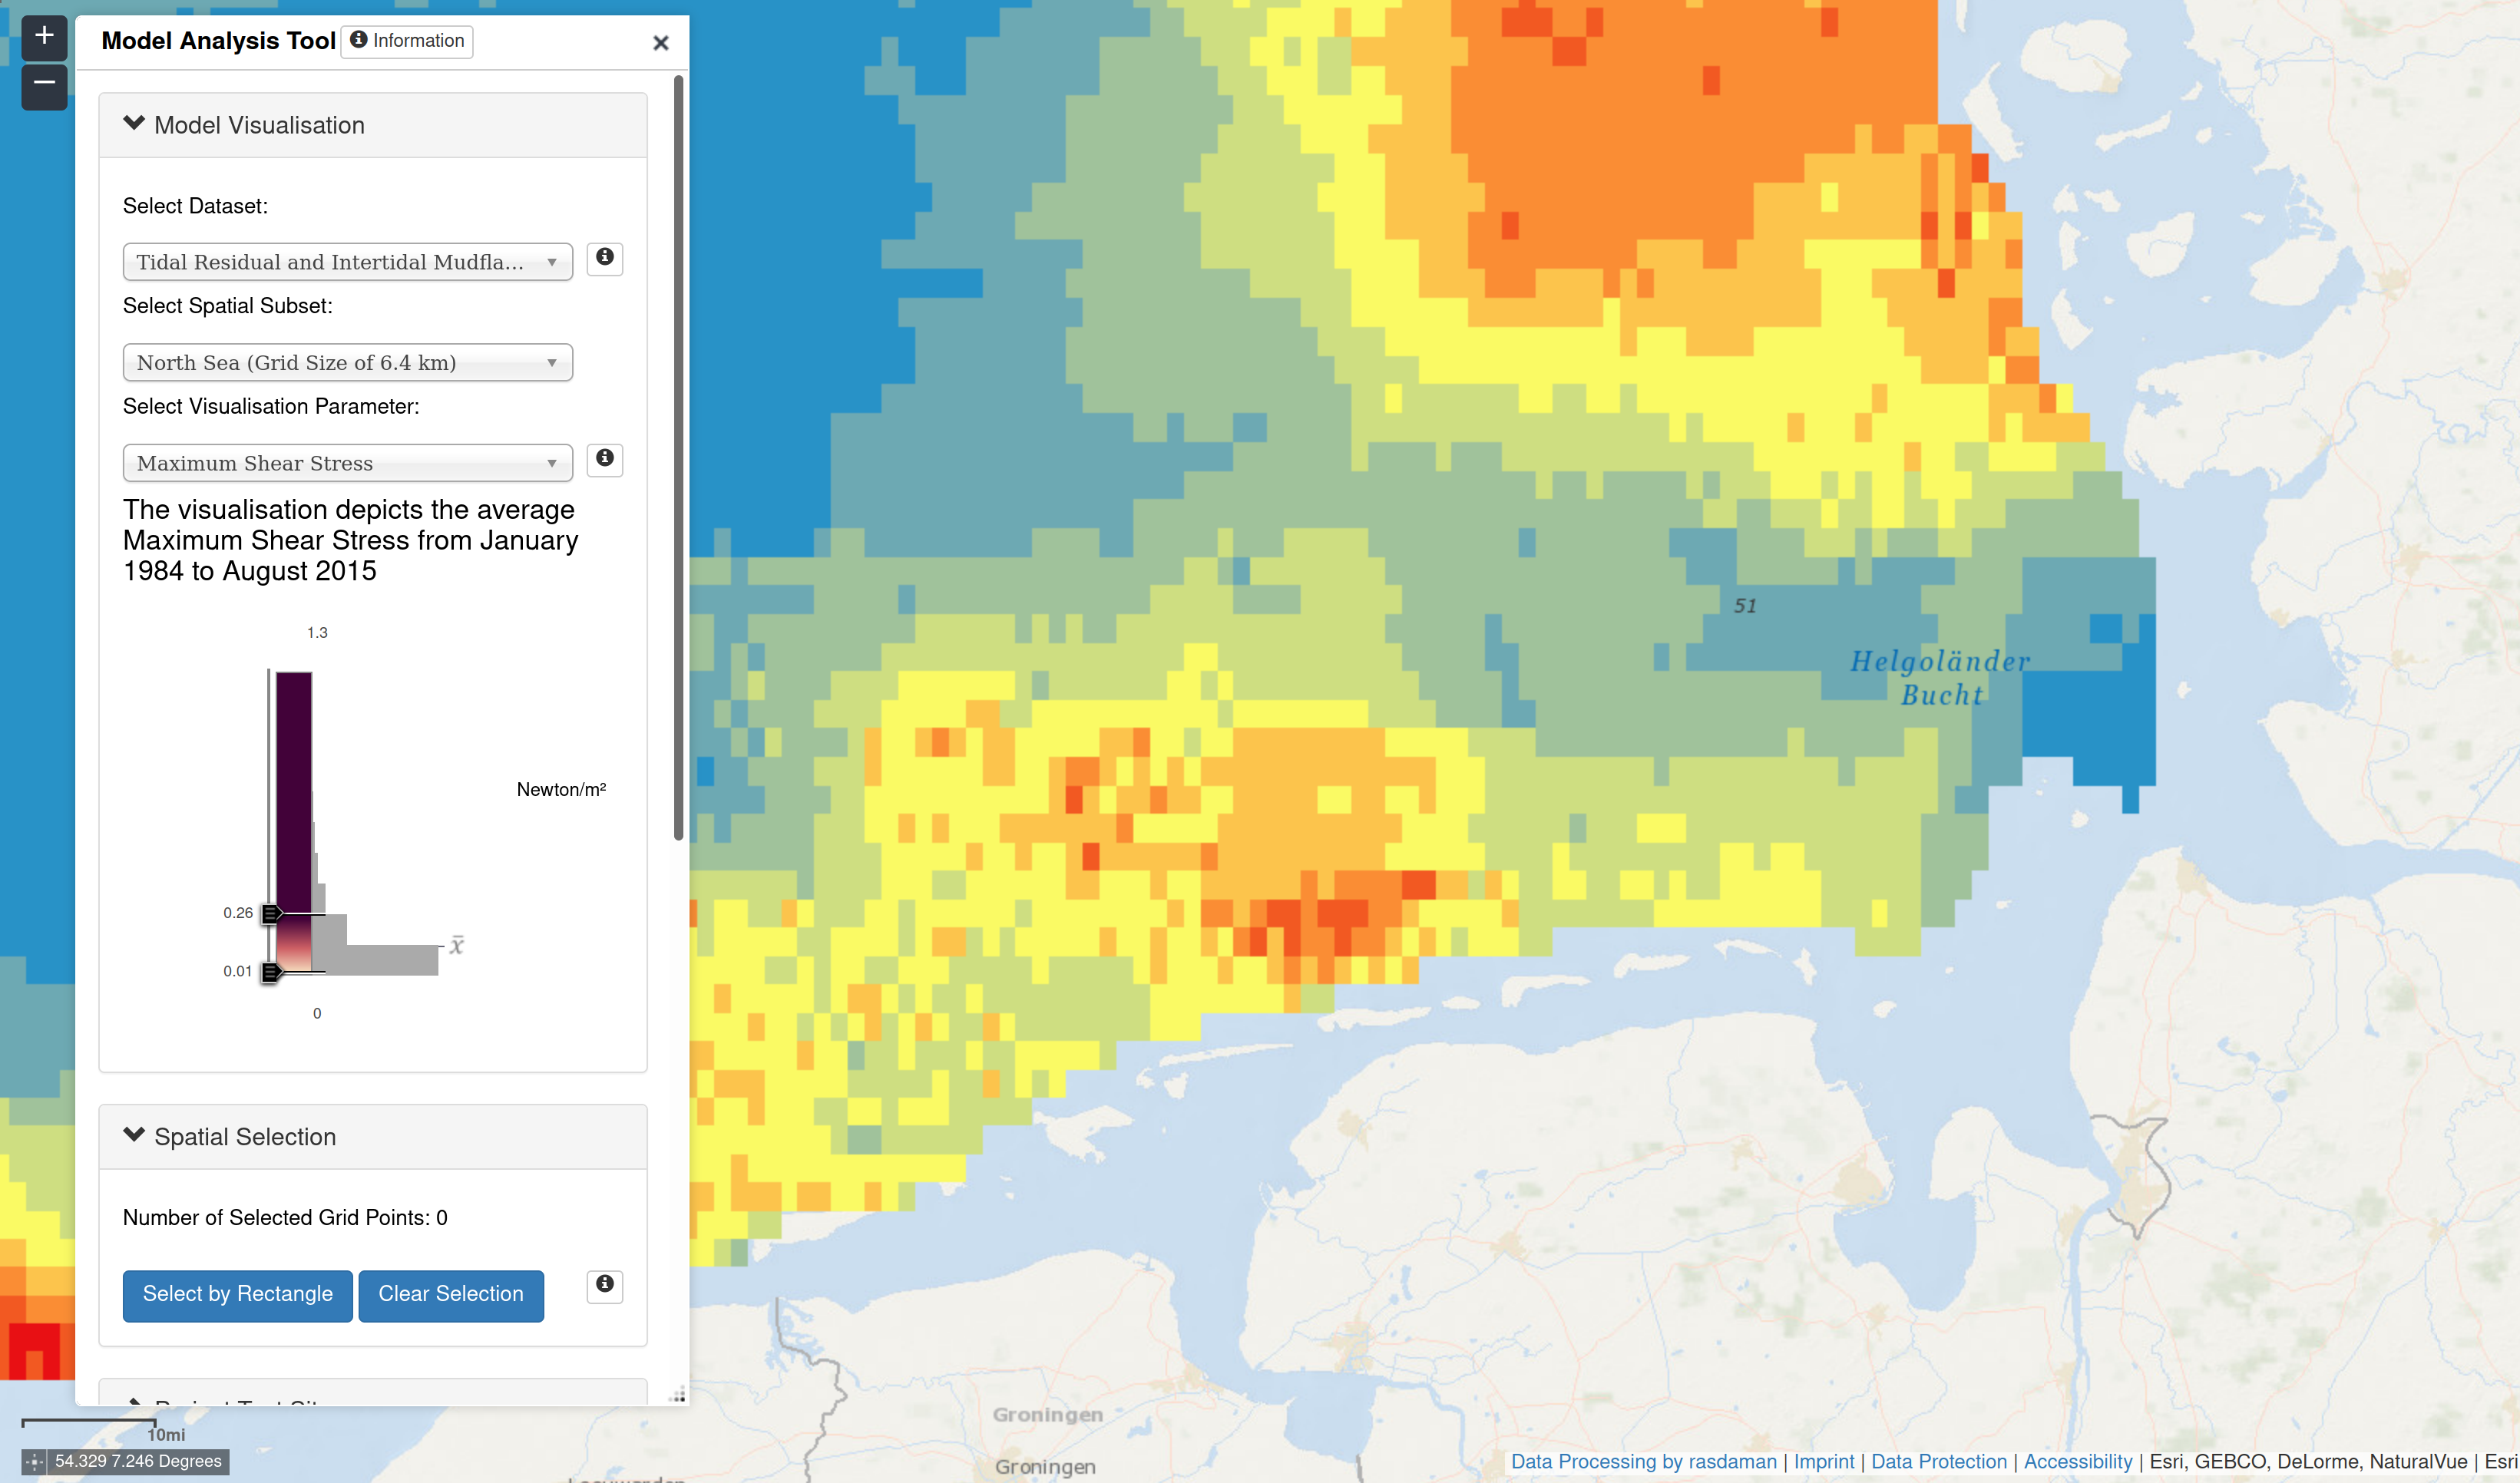
\includegraphics[width=\textwidth]{figures/demo-screenshot-model-data-explorer.png}
            \end{column}
        \end{columns}
    \end{block}
\end{frame}

\subsection*{Service Plugins}

\begin{frame}{A modular and federated system}
    \begin{columns}
        \begin{column}{0.3\textwidth}
            \begin{itemize}
                \item Single configuration interface for multiple connected
                    services
                \item multiple standard interfaces
                \item Federation to connect multiple research centers
            \end{itemize}

            \vspace{1em}

            \hyperlink{frm:service-plugins}{\beamerbutton{\normalsize More \ldots}}
        \end{column}
        \begin{column}{0.7\textwidth}
            \includegraphics[width=\textwidth, page=2]{figures/mde-service-plugins-basic.pdf}
        \end{column}
    \end{columns}
\end{frame}
% !TeX root = ../mde-presentation.tex

\section{Authors}  \label{sec:authors}

\begin{frame}{Author}
	\label{frm:author}
	\begin{columns}[T]
		\begin{column}{0.7\linewidth}
			\begin{block}{Philipp S. Sommer}
				Helmholtz Coastal Data Center (HCDC) \\
				Helmholtz-Zentrum hereon GmbH \\
				Max-Planck-Straße 1 \\
				DE - 21502 Geesthacht \\
				\vspace{0.5em}
				\begin{description}
					\item[E-mail] \href{mailto:\authoremail}{\authoremail}
					\item[Telefon] +49 4152 87 2126
					\item[Github] \url{https://github.com/Chilipp}
					\item[Webpage] \url{https://www.philipp-s-sommer.de}
				\end{description}
				\hyperlink{frm:map}{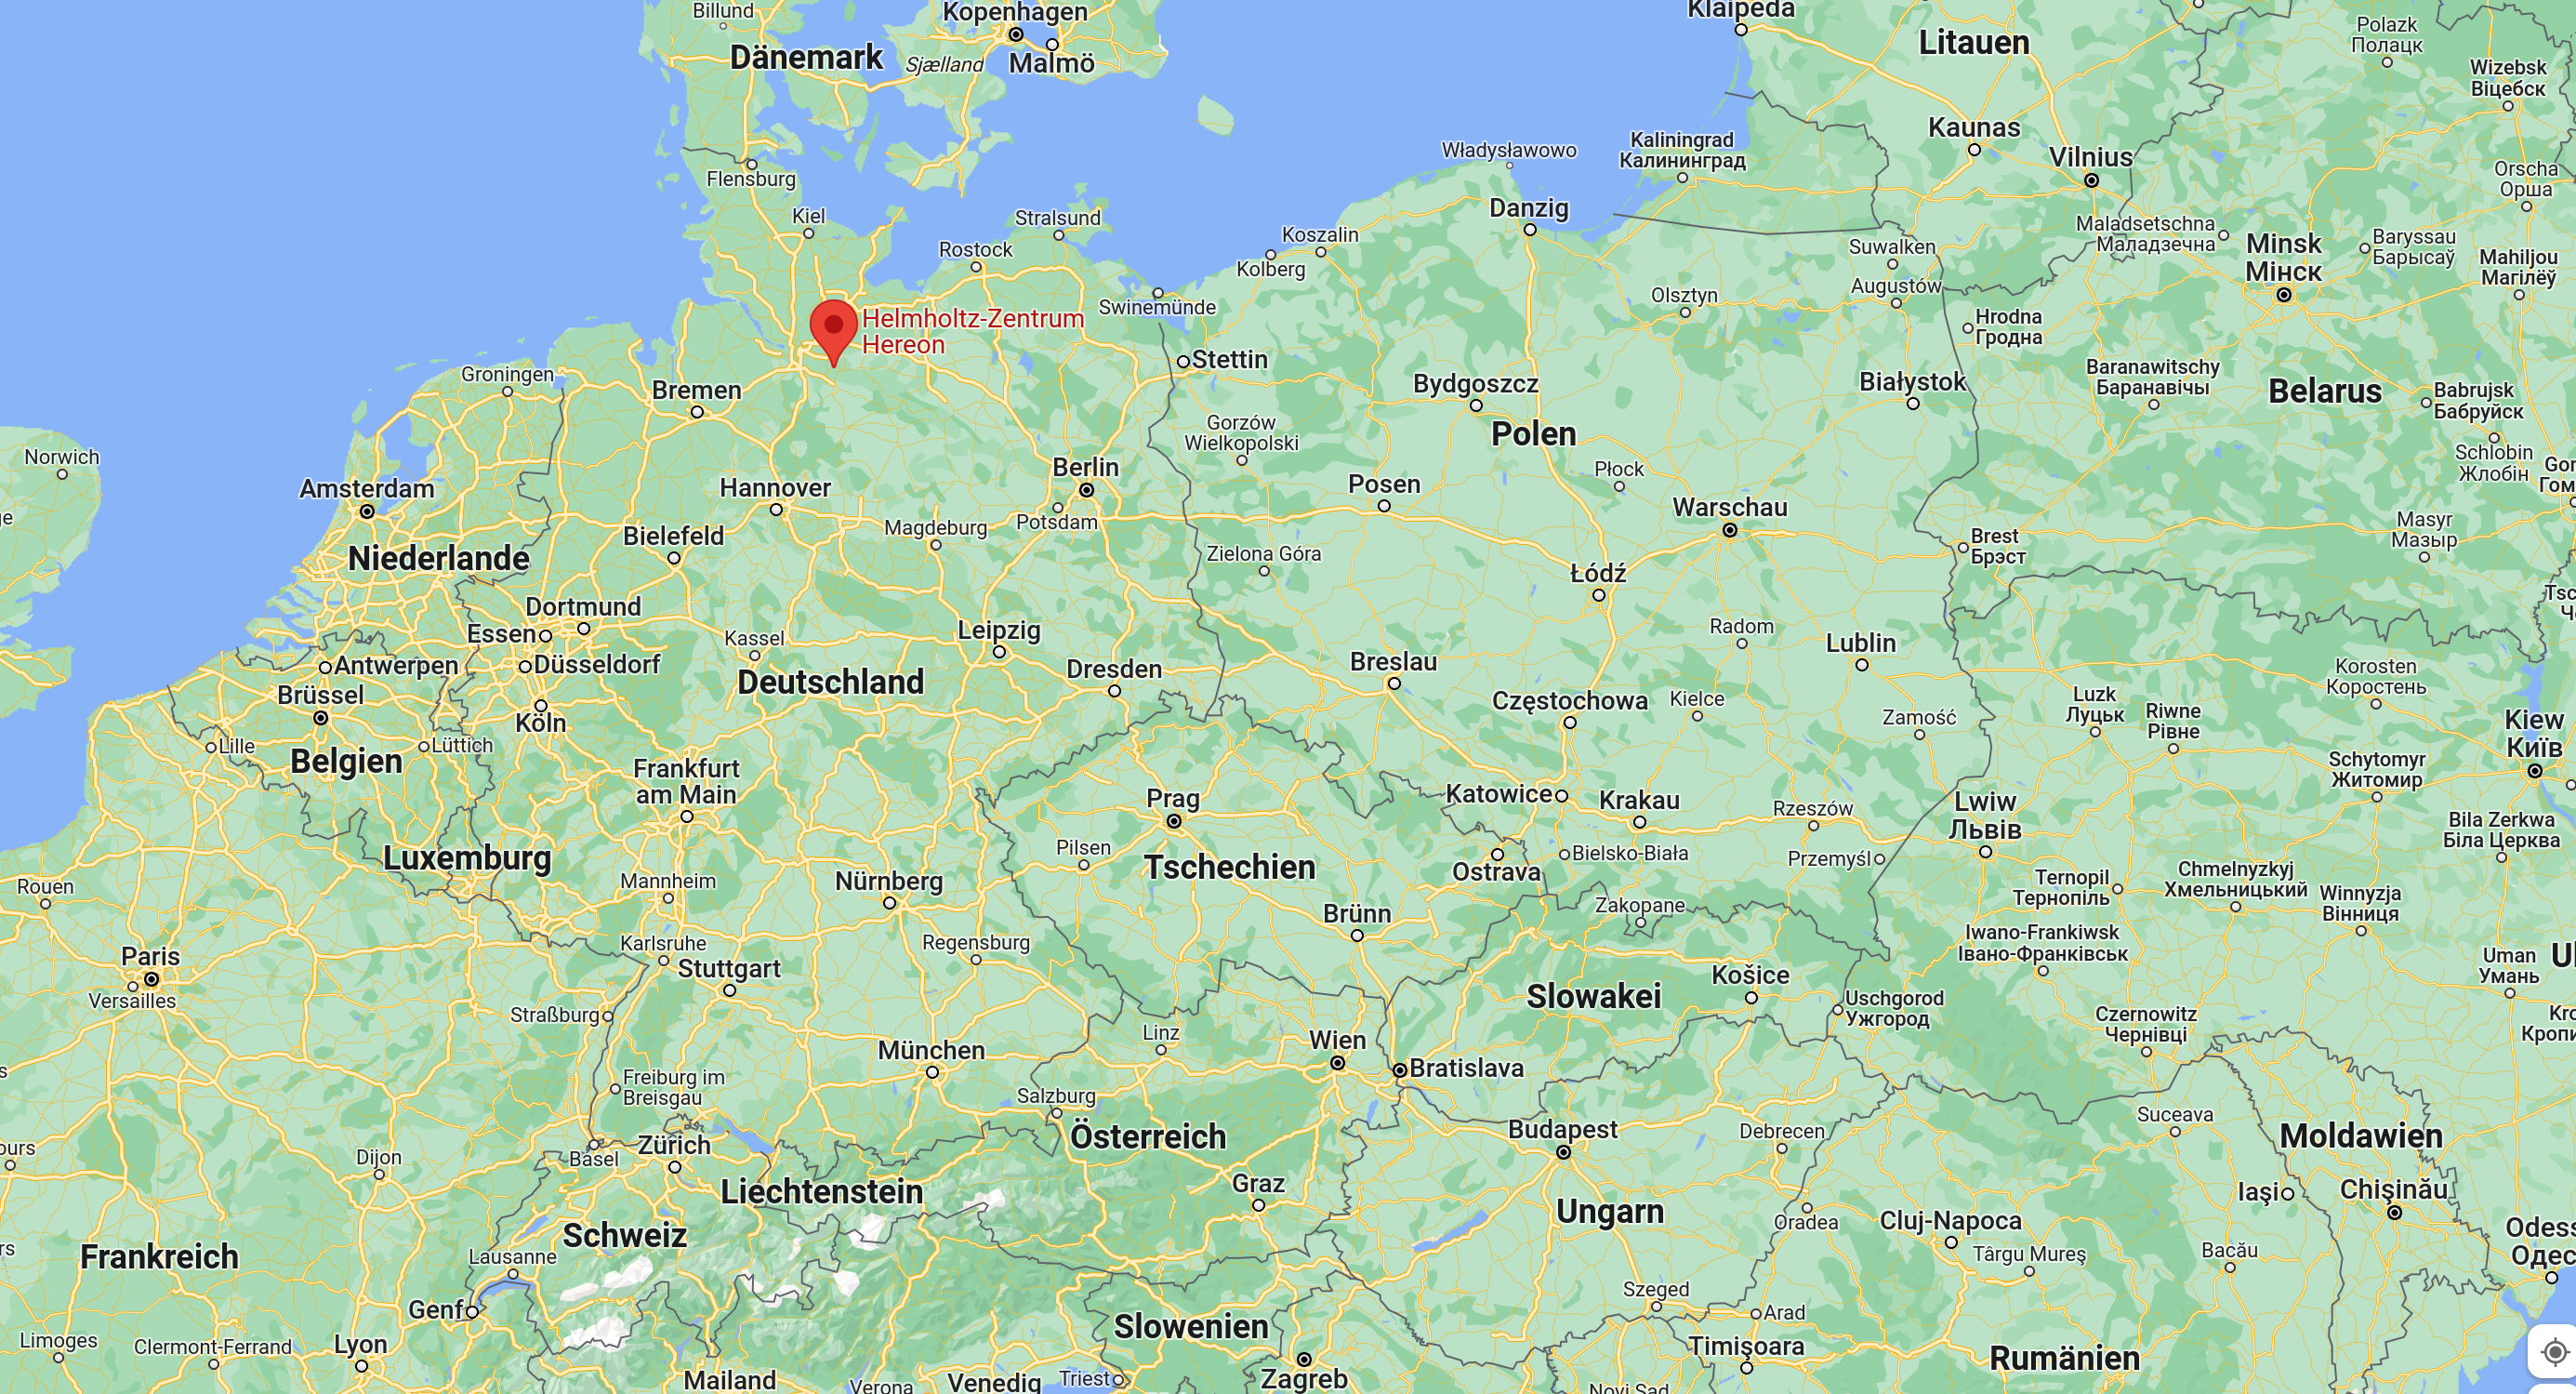
\includegraphics[width=0.25\linewidth]{figures/hereon-map.png}}
			\end{block}
		\end{column}
		\begin{column}{0.25\linewidth}
			
\includegraphics[width=\linewidth]{figures/psommer.jpg}
		\end{column}
	\end{columns}
\end{frame}

\begin{frame}{Co-Authors}

	\begin{columns}[T]
		\begin{column}{0.5\linewidth}

			\begin{block}{Helmholtz-Zentrum Hereon}
				\begin{itemize}
					\item Linda Baldewein
					\item Hatef Takyar
					\item Rehan Chaudhary
					\item Housam Dibeh
					\item Max Böcke
					\item Ulrike Kleeberg
				\end{itemize}
				\vspace{1em}
				\qquad \href{https://www.hereon.de}{
					
\includegraphics[width=0.4\linewidth]{figures/hereon.png}
				}
			\end{block}
		\end{column}

		\begin{column}{0.5\linewidth}
			\begin{block}{Karlsruhe Institute of Technology}
				\begin{itemize}
					\item Mostafa Hadizadeh
					\item Christof Lorenz
				\end{itemize}
			\end{block}

			\begin{block}{Alfred-Wegener-Institut}
				\begin{itemize}
					\item Tilman Dinter
					\item Stefan Pinkernell
				\end{itemize}
			\end{block}

			\begin{block}{Geomar}
				\begin{itemize}
					\item Klaus Getzlaff
				\end{itemize}
			\end{block}

		\end{column}
	\end{columns}

	\vspace{1em}

	\begin{columns}[T]
		\begin{column}{0.3\linewidth}
			\centering
			\href{https://www.awi.de}{
				
\includegraphics[width=0.5\linewidth]{figures/awi_logo.pdf}
			} \\
			\vspace{1em}
			\href{https://www.geomar.de}{
				
\includegraphics[width=0.5\linewidth]{figures/geomar_logo.pdf}
			}
		\end{column}

		\begin{column}{0.3\linewidth}
			\centering
			\href{https://datahub.erde-und-umwelt.de}{
				
\includegraphics[width=0.5\linewidth]{figures/datahub.png}
			 } \\
			\vspace{1em}
			\href{https://www.helmholtz.de/}{
				
\includegraphics[width=0.5\linewidth]{figures/helmholtz.pdf}
			}

		\end{column}

		\begin{column}{0.3\linewidth}
			\centering
			\href{https://kit.edu}{
				
\includegraphics[width=0.5\linewidth]{figures/kit.pdf}
			 } \\
			 \vspace{1em}
			 \href{https://kit.edu}{
				 
\includegraphics[width=0.5\linewidth]{figures/cat4kit.png}
			  }
		\end{column}
	\end{columns}

\end{frame}

\subsection*{Funding} \label{sec:funding}

\begin{frame}{Funding}
	\begin{columns}[T]

		\begin{column}{0.7\linewidth}
			The conceptualization of the Model Data Explorer has been made
			possible through the DataHub funding. Initial developments for
			the THREDDS-Server management are funded through Cat4KIT.

			We hope to get funding through an NFDI4Earth Pilot
			(\url{https://www.nfdi4earth.de/}) for the core implementation
			of the model data explorer.

			\vspace{2.3em}
			\begin{flushright}
				\fcolorbox{hereondarkblueshaded}{white}{
					\begin{tabular}{@{}r@{}}
						\href{https://www.nfdi4earth.de/}{
							
\includegraphics[width=0.4\linewidth]{figures/NFDI4Earth_logo.png}
						} \\
						\textit{\footnotesize *Proposal submitted}
					\end{tabular}
				}
			\end{flushright}
		\end{column}

		\begin{column}{0.3\linewidth}
			\href{https://www.helmholtz.de/}{
				
\includegraphics[width=\linewidth]{figures/helmholtz.pdf}
			} \\
			\vspace{1em}
			\href{https://datahub.erde-und-umwelt.de}{
				
\includegraphics[width=\linewidth]{figures/datahub.png}
			} \\
			\vspace{1em}
			\href{https://kit.edu}{
				
\includegraphics[width=0.5\linewidth]{figures/cat4kit.png}
			}
		\end{column}
	\end{columns}
\end{frame}

% !TeX root = ../mde-presentation.tex

\section{Abstract} \label{sec:abstract}

\begin{frame}[t, allowframebreaks]{Abstract}
	\begin{block}{ESM Data Exploration with the Model Data Explorer}
		\begin{small}
			Making Earth-System-Model (ESM) Data accessible is challenging due
			to the large amount of data that we are facing in this realm. The
			upload is time-consuming, expensive, technically complex, and every
			institution has their own procedures.

            Non-ESM experts face a lot of problems and pure data portals are
			hardly usable for inter- and trans-disciplinary communication of
			ESM data and findings, as this level of accessibility often
			requires specialized web or computing services.

            With the Model Data Explorer, we want to simplify the generation of
			web services from ESM data, and we provide a framework that allows
			us to make the raw model data accessible to non-ESM experts.

            Our decentralized framework implements the possibility for an
			efficient remote processing of distributed ESM data. Users
			interface with an intuitive map-based front-end to compute spatial
			or temporal aggregations, or select regions to download the data.
			The data generators (i.e. the scientist with access to the raw
			data) use a light-weight and secure python library based on the
			Data Analytics Software Framework (DASF,
			\url{https://digital-earth.pages.geomar.de/dasf/dasf-messaging-python})
			to create a back-end module. This back-end module runs close to the
			data, e.g. on the HPC-resource where the data is stored. Upon
			request, the module generates and provides the required data for
			the users in the web front-end.

		\end{small}
	\end{block}

	\framebreak

	\begin{block}{ESM Data Exploration with the Model Data Explorer}
		\begin{small}
            Our approach is intended for scientists and scientific usage! We
			aim for a framework where web-based communication of model-driven
			data science can be maintained by the scientific community. The
			Model Data Explorer ensures fair reward for the scientific work and
			adherence to the FAIR principles without too much overhead and loss
			in scientific accuracy.

            The Model Data Explorer is in the progress of development at the
			Helmholtz-Zentrum Hereon, together with multiple scientific and
			data management partners in other German research centers. The full
			list of contributors is constantly updated and can be accessed at
			\url{https://model-data-explorer.readthedocs.io}.

		\end{small}
	\end{block}
\end{frame}


% !TeX root = ../mde-presentation.tex

\section{Implementation} \label{sec:implementation}

\subsection*{Core} \label{sec:core}

\begin{frame}{Core} \label{frm:core}

    \begin{columns}[T]
        \begin{column}{0.4\textwidth}
            \only<1>{
                The core package of the Model Data Explorer,
                \lstinline|mde-core|, implemented with Django, implements
                so-called \textit{Datasets}. A dataset might be identified
                with a specific experiment to run a model. It gets a unique
                handle and UUID and serves as a kind of namespace for the
                services associated with it. This makes resources related to a
                dataset better findeable as everything is linked to a specific
                dataset.
            }

            \only<2>{

                \lstinline|mde-core| additionally implements data groups.
                This can be anything from a project to a department or an
                institution. DataGroups can own datasets and they will be listed
                on their detail page. DataGroups can also own other DataGroups and
                as such inherit ownerships on the datasets.

                \lstinline|mde-core| uses a directed acyclic graph implementation
                \citep{OmenApps2021} to efficiently manage data group relations
                and permissions.
            }


        \end{column}
        \begin{column}{0.55\textwidth}
            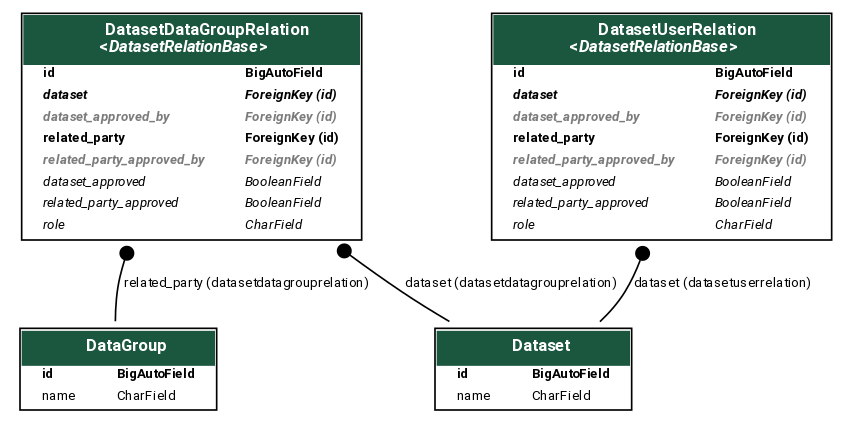
\includegraphics[width=\textwidth]{figures/dataset-datagroup.png}
            \only<2>{
                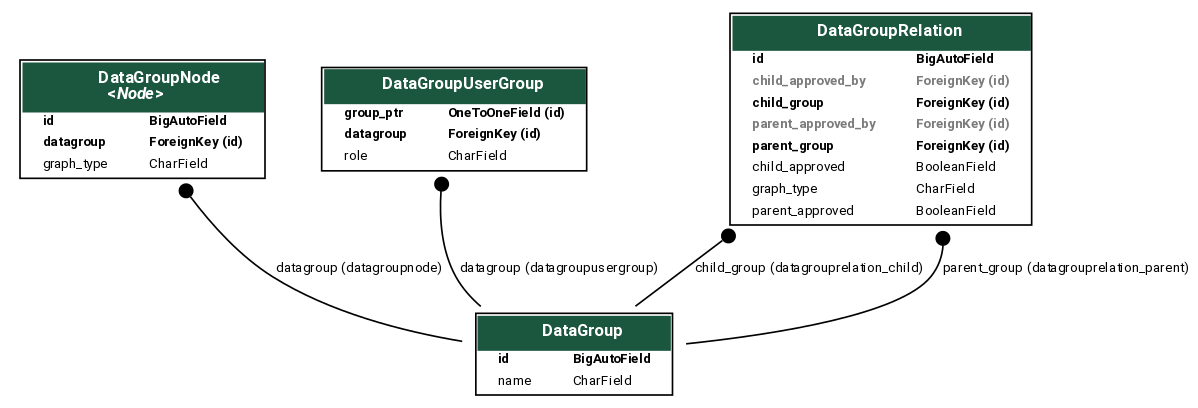
\includegraphics[width=\textwidth]{figures/datagroup-implementation.png}
            }
        \end{column}

    \end{columns}

    \begin{textblock*}{\textwidth}(0.05\linewidth, 1.07\textheight)
		\slidebuttons
	\end{textblock*}

\end{frame}

\begin{frame}{DataGroup relations}

    \label{frm:datagroup-relations}

    \begin{columns}[T]
        \begin{column}{0.4\textwidth}
            \begin{block}{In Research}
                \begin{itemize}
                    \item Many partners are involved in different projects
                    \item Data managers need to be able to configure metadata and create services
                    \item Relations should be built from the metadata and vice-versa
                \end{itemize}
            \end{block}
        \end{column}
        \begin{column}{0.55\textwidth}
            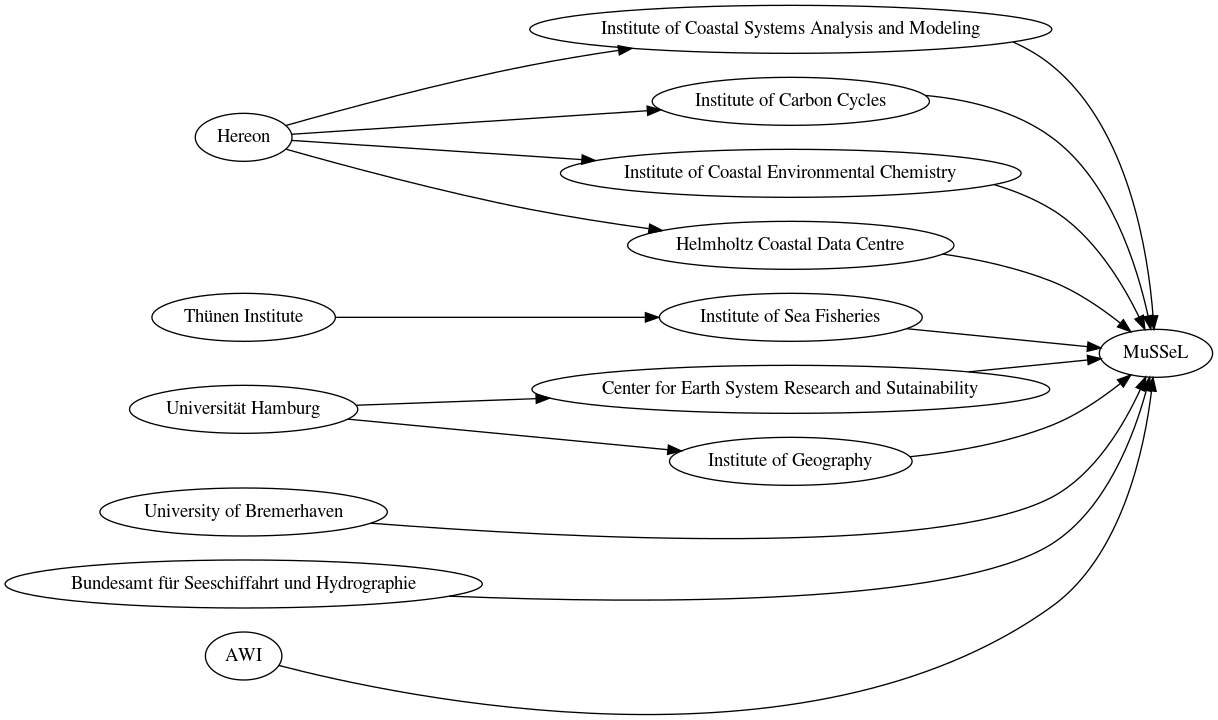
\includegraphics[width=\textwidth]{figures/datagroup-tree.png}
        \end{column}

    \end{columns}

    \begin{block}{In the Model Data Explorer}
        \vspace{0.5em}
        \begin{tabular}{p{0.5\textwidth}p{0.5\textwidth}}
            \tabitem Relationships between groups are
                \par \hspace{1.5ex} represented with a directed acyclic graph &
            \tabitem \indent Each institute, department, unit, project,
                \par \hspace{1.5ex} etc. gets its own page \\
            \tabitem Datasets are shown on each group site &
            \tabitem Maintainability is guaranteed through data
                \par \hspace{1.5ex} group relations
        \end{tabular}
    \end{block}

\end{frame}
% !TeX root = ../mde-presentation.tex

\subsection*{Plugins} \label{sec:plugins}

\begin{frame}{Plugins}
    \label{frm:plugins}
    Each research center has a different IT infrastructure and works with
    different frameworks. The aim of the model data explorer is to integrate
    these different systems into a user-friendly web-application. In order to
    be able to deploy the model data explorer at the different research
    centers, we aim for a modular structure where each component can be added
    or removed depending on the setup at the hosting institution.

    This modular structure is implemented via plugins. Each plugin is a python
    package containing a django app that can be added or removed from the
    configuration. We distinguish between three plugin categories:
    \hyperlink{frm:core}{core},
    \hyperlink{frm:framework-plugins}{framework} and
    \hyperlink{frm:service-plugins}{service} plugins.

    \vspace{2em}

    \begin{center}
        \begin{tabular}{p{0.4\textwidth}p{0.2\textwidth}p{0.3\textwidth}}
            \hyperlink{frm:framework-plugins}{\beamerbutton{\Large Framework plugins}} \\
            & \hyperlink{frm:core}{\beamerbutton{\Large Core}} \\
            & & \hyperlink{frm:service-plugins}{\beamerbutton{\Large Service plugins}}
        \end{tabular}
    \end{center}
\end{frame}

\begin{frame}{Framework plugins} \label{frm:framework-plugins}
    Framework plugins contain optionally but commonly used features for service
    plugins and are independent of the IT infrastructure.

    \begin{columns}[T]
        \begin{column}{0.45\textwidth}
            \begin{block}{mde-config}
                \begin{itemize}
                    \item defines a viewset-based structure where service
                        plugins can provide configuration interfaces for
                        individual datasets.
                    \item provides user configuration interfaces for the
                        \lstinline|mde-core| models.
                \end{itemize}
            \end{block}
            \begin{block}{mde-federation}
                \begin{itemize}
                    \item combines multiple MDE instances at different
                        institutions.
                    \item synchronizes datasets and data groups between
                        independant instances
                \end{itemize}
                \hyperlink{frm:federation}{\beamerbutton{Read more \ldots}}

            \end{block}
        \end{column}
        \begin{column}{0.45\textwidth}
            \begin{block}{mde-notifications}
                \begin{itemize}
                    \item implements the functionalities to send out
                        notifications to the users (e.g. for confirmations
                        required by dataset or data group owners)
                    \item provides an interface for the user for configuring
                        notifications
                \end{itemize}
            \end{block}

            \begin{block}{mde-oauth}
                \begin{itemize}
                    \item implements the possibility for the model data
                        explorer to serve as an OAuth or SAML Provider
                    \item gives attached services the possibility to
                        authenticate against the MDE and get
                        the users groups.
                \end{itemize}
            \end{block}
        \end{column}
    \end{columns}
\end{frame}

\begin{frame}{Service plugins} \label{frm:service-plugins}
    \begin{columns}
        \begin{column}{0.3\textwidth}
            Service plugins are based on the available IT infrastructure at a
            research institution. They connect a dataset of the
            \lstinline|mde-core| to an external service. This way, the MDE is
            configuring this external service.

            Service plugins should be independent of other service plugins (if
            possible) but they can depend on one of the
            \hyperlink{frm:framework-plugins}{framework plugins}.
        \end{column}
        \begin{column}{0.7\textwidth}
            \includegraphics[width=\textwidth, page=3]{figures/mde-service-plugins-basic.pdf}
        \end{column}
    \end{columns}
\end{frame}

\begin{frame}[t]{Planned service plugins}
    \begin{columns}[T]
        \begin{column}{0.45\textwidth}
            \only<1>{
                \begin{block}{mde-viewer}
                    A map-based viewer frontend for a dataset based on
                    ArcGIS4Javascript and angular. It displays all metadata and
                    services for an individual dataset. Services that are displayed
                    in this viewer are configured through the mde-esri,
                    mde-thredds, mde-analysis and mde-download plugins.
                \end{block}
                \begin{block}{mde-thredds}
                    This app creates catalog and configuration files for a
                    THREDDS-Server \citep{Caron1997} and restarts it when the
                    configuration changed.
                \end{block}
            }
            \only<2>{
                \begin{block}{mde-analysis}
                    The Analysis framework for the model data explorer.
                    Based upon the Data Analytics Software Framework
                    \citep[DASF, ][]{Eggert2022}
                    this plugin provides the framework to compute aggregated
                    analysis on datasets without the need to download the raw
                    data.
                \end{block}
            }
        \end{column}
        \begin{column}{0.45\textwidth}
            \only<1>{
                \begin{block}{mde-mams}
                    At Hereon, AWI and Geomar, we host instances of the
                    \textit{Media Assets Management System}, also called MAMS.
                    Through \lstinline|mde-mams|, users can request storage in
                    MAMS to upload netCDF files.
                    These workspaces are additionally mounted on the THREDDS-Server.
                \end{block}

                \begin{block}{mde-csw}
                    The \lstinline|mde-csw| plugin can combine multiple ISO-files
                    (e.g. generated via THREDDS) and provides an OGC-compliant CSW
                    endpoint via pycsw \citep{Kralidis2023}.
                \end{block}
            }
            \only<2>{
                \begin{block}{mde-download}
                    The download framework for the model data explorer. As
                    \lstinline|mde-analysis| based upon the DASF. This plugin
                    provides the framework to download subsets of the data.
                \end{block}
            }
        \end{column}
    \end{columns}

    \only<2>{
        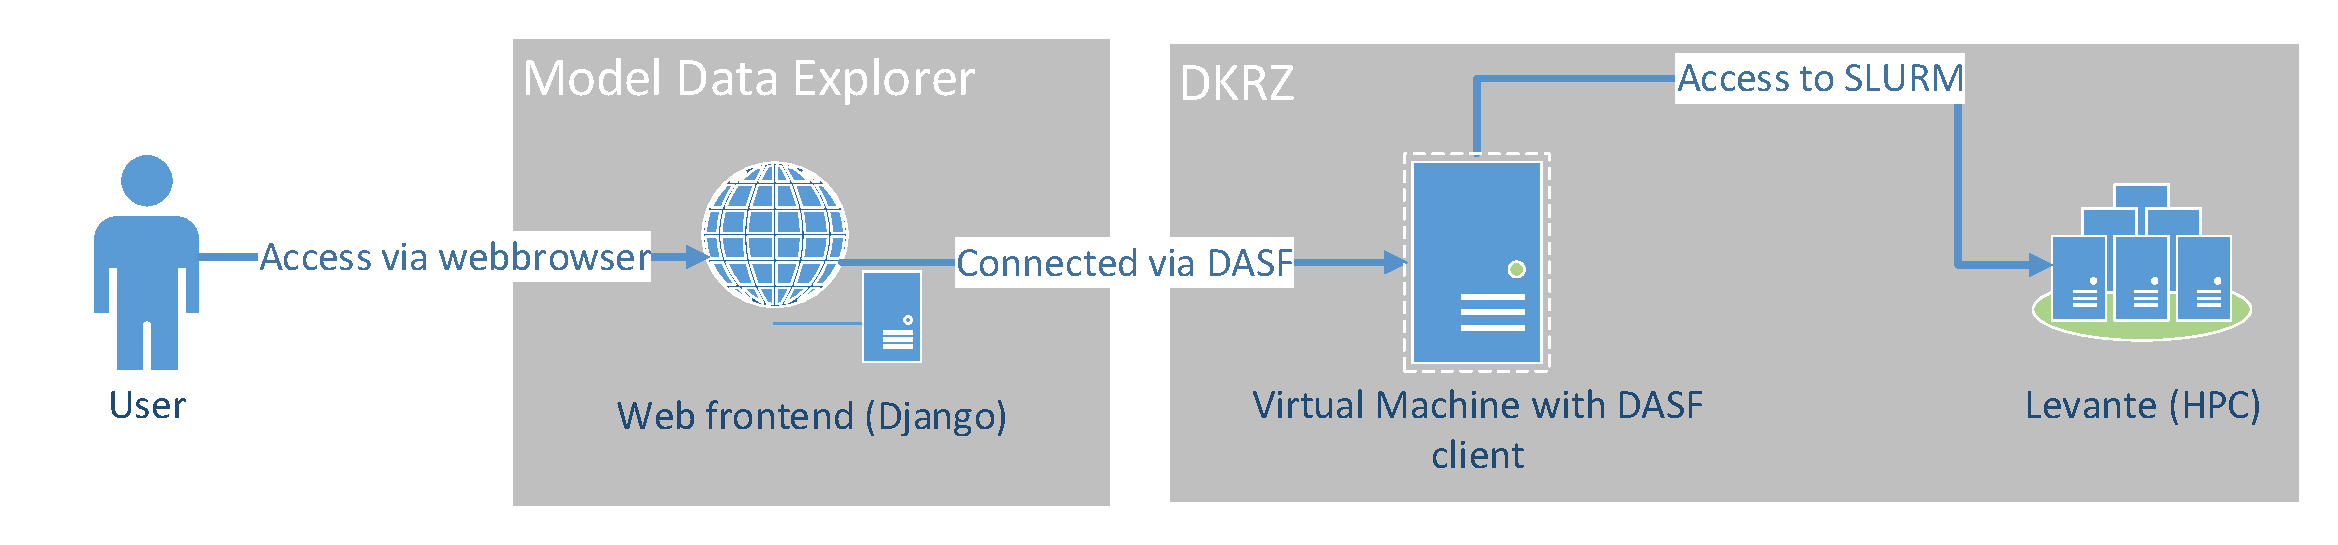
\includegraphics[width=\textwidth]{figures/dasf-schema.pdf}
    }

    \begin{textblock*}{\textwidth}(0.05\linewidth, 1.07\textheight)
		\slidebuttons
	\end{textblock*}

\end{frame}
% !TeX root = ../mde-presentation.tex

\subsection*{Federation} \label{sec:federation}

\begin{frame}{Federation} \label{frm:federation}

    A core concept within the model data explorer is the federation between
    multiple MDE instances. This is essential as multiple institutions might
    offer different services for one single dataset. One institution might make
    the data available via THREDDS, the other one might make it available as
    ESRI \lstinline|ImageService|.

    \begin{columns}
        \begin{column}{0.45\textwidth}
            \begin{block}{Core concepts}
                \begin{enumerate}
                    \item Each data groups has a unique hosting MDE
                    \item OAuth for synchronizing user permissions between two MDE instances
                    \item A websocket messaging for synchronizing MDE instances
                \end{enumerate}
            \end{block}
        \end{column}
        \begin{column}{0.45\textwidth}
            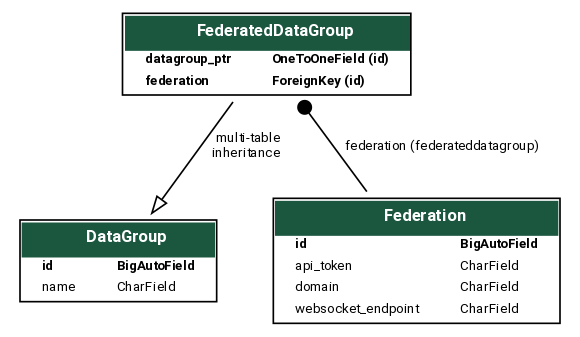
\includegraphics[width=\textwidth]{figures/mde-federation-models.png}
        \end{column}
    \end{columns}

\end{frame}

\begin{frame}{Websocket implementation for federation}

    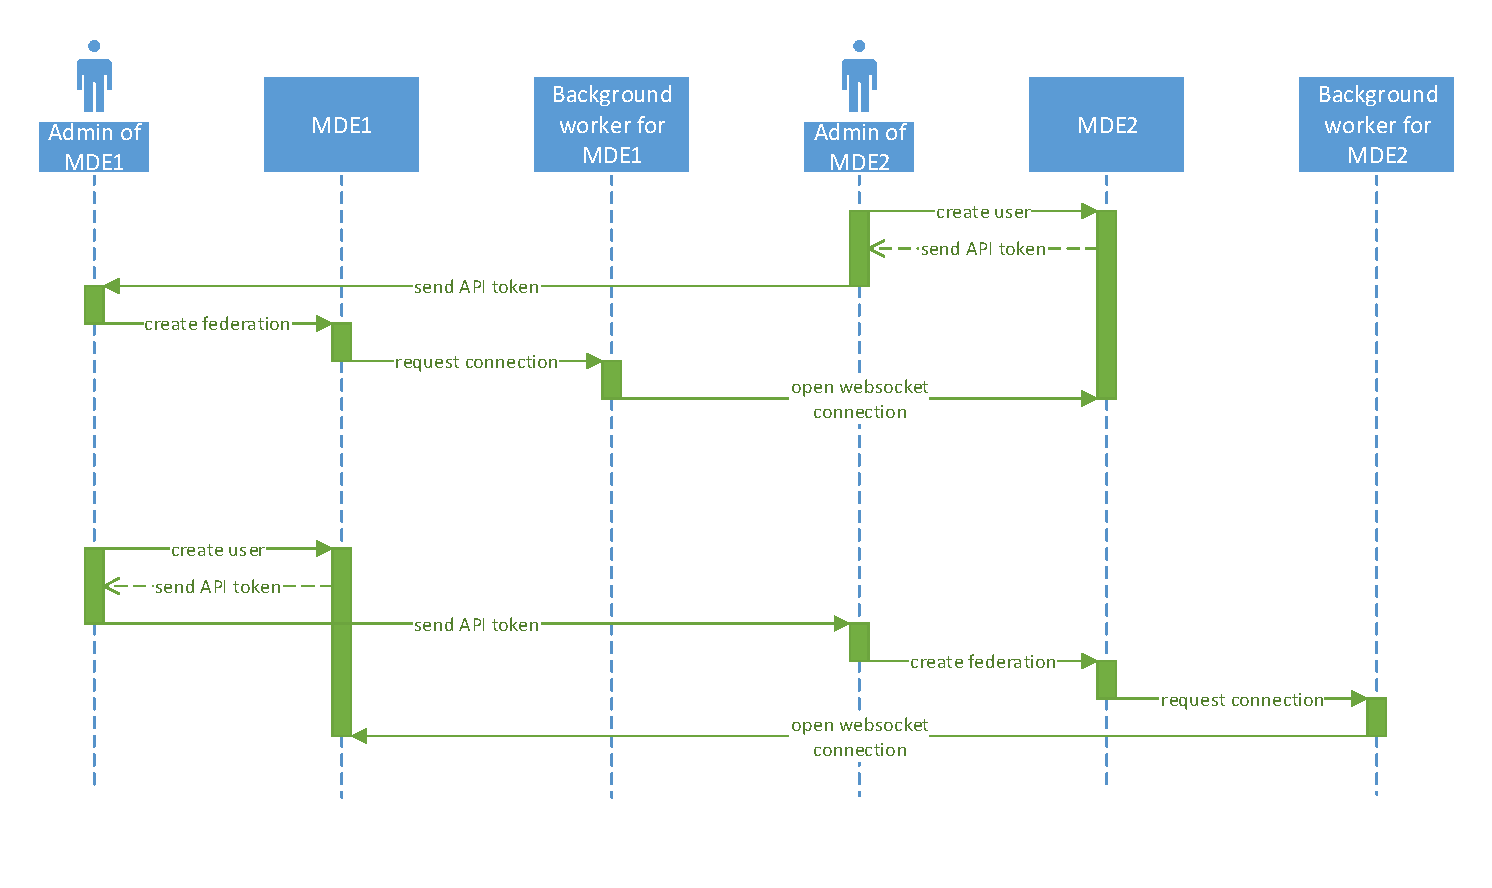
\includegraphics[width=\textwidth]{figures/mde-federation.pdf}

\end{frame}
% !TeX root = ../mde-presentation.tex

\section{Maintenance} \label{sec:maintenance}

\begin{frame}[t]{Maintenance}

    \begin{columns}
        \begin{column}{0.6\textwidth}
            \begin{block}{Templating, Packaging and Containerization}
                We plan to systemize and guarantee maintenance through a
                sophisticated templating mechanism for generating and updating
                plugins and docker-based deployments with
                \href{https://github.com/cruft/cruft}{cruft} and
                \href{https://github.com/cookiecutter/cookiecutter}{cookiecutter}.

                Standardized and flexible deployments will be implemented with
                helm charts for kubernetes and openshift.
            \end{block}

            \vspace{1em}

            \href{https://de-rse.org}{
                
\includegraphics[width=0.5\textwidth]{figures/BetterSoftwareBetterResearchImage.jpg}
            }

        \end{column}
        \begin{column}{0.4\textwidth}
            \href{https://github.com/cruft/cruft}{
                
\includegraphics[width=0.45\textwidth]{figures/cruft.png}
            }
            \href{https://codebase.helmholtz.cloud/model-data-explorer/}{
                
\includegraphics[width=0.45\textwidth]{figures/gitlab-logo.pdf}
            } \\
            \vspace{1em}
            
\includegraphics[width=0.45\textwidth]{figures/Kubernetes_logo.svg.png}
            
\includegraphics[width=0.45\textwidth]{figures/openshift.png} \\
            \vspace{1em}
            
\includegraphics[width=0.45\textwidth]{figures/docker-logo.png} \\
        \end{column}
    \end{columns}

\end{frame}
% !TeX root = ../mde-presentation.tex

\section{Resources} \label{sec:resources}

\begin{frame}[t]{Resources}

    \begin{columns}[T]
        \begin{column}{0.5\textwidth}
            \begin{block}{Documentation}
                \begin{small}
                    \url{https://model-data-explorer.readthedocs.io/projects/prototype/} \\
                \end{small}
                \href{https://model-data-explorer.readthedocs.io/projects/prototype/}{
                    
\includegraphics[width=4cm]{figures/qrcode-rtd-prototype.png}
                }
            \end{block}
        \end{column}
        \begin{column}{0.45\textwidth}
            \begin{block}{Source Code}
                \begin{small}
                    \url{https://codebase.helmholtz.cloud/model-data-explorer/} \\
                \end{small}
                \href{https://codebase.helmholtz.cloud/model-data-explorer/}{
                    
\includegraphics[width=4cm]{figures/qrcode-gitlab.png}
                }
            \end{block}
        \end{column}
    \end{columns}

    \begin{block}{Presentation material}
        \begin{small}
            \url{https://github.com/Chilipp/mde-presentation-egu2023} \\
        \end{small}
        \href{https://github.com/Chilipp/mde-presentation-egu2023}{
            
\includegraphics[width=4cm]{figures/qrcode-presentation.png}
        }
    \end{block}

\end{frame}

%Appendix
\appendix

%Bibliography
\section{Appendix}
\subsection{References}
\begin{frame}[allowframebreaks]{References}{}

% \begin{tiny}
\bibliographystyle{abbrvnat}
\bibliography{references}
% \end{tiny}
\end{frame}

\begin{frame}
\frametitle[Hereon]{Helmholtz-Zentrum Hereon}
\label{frm:map}
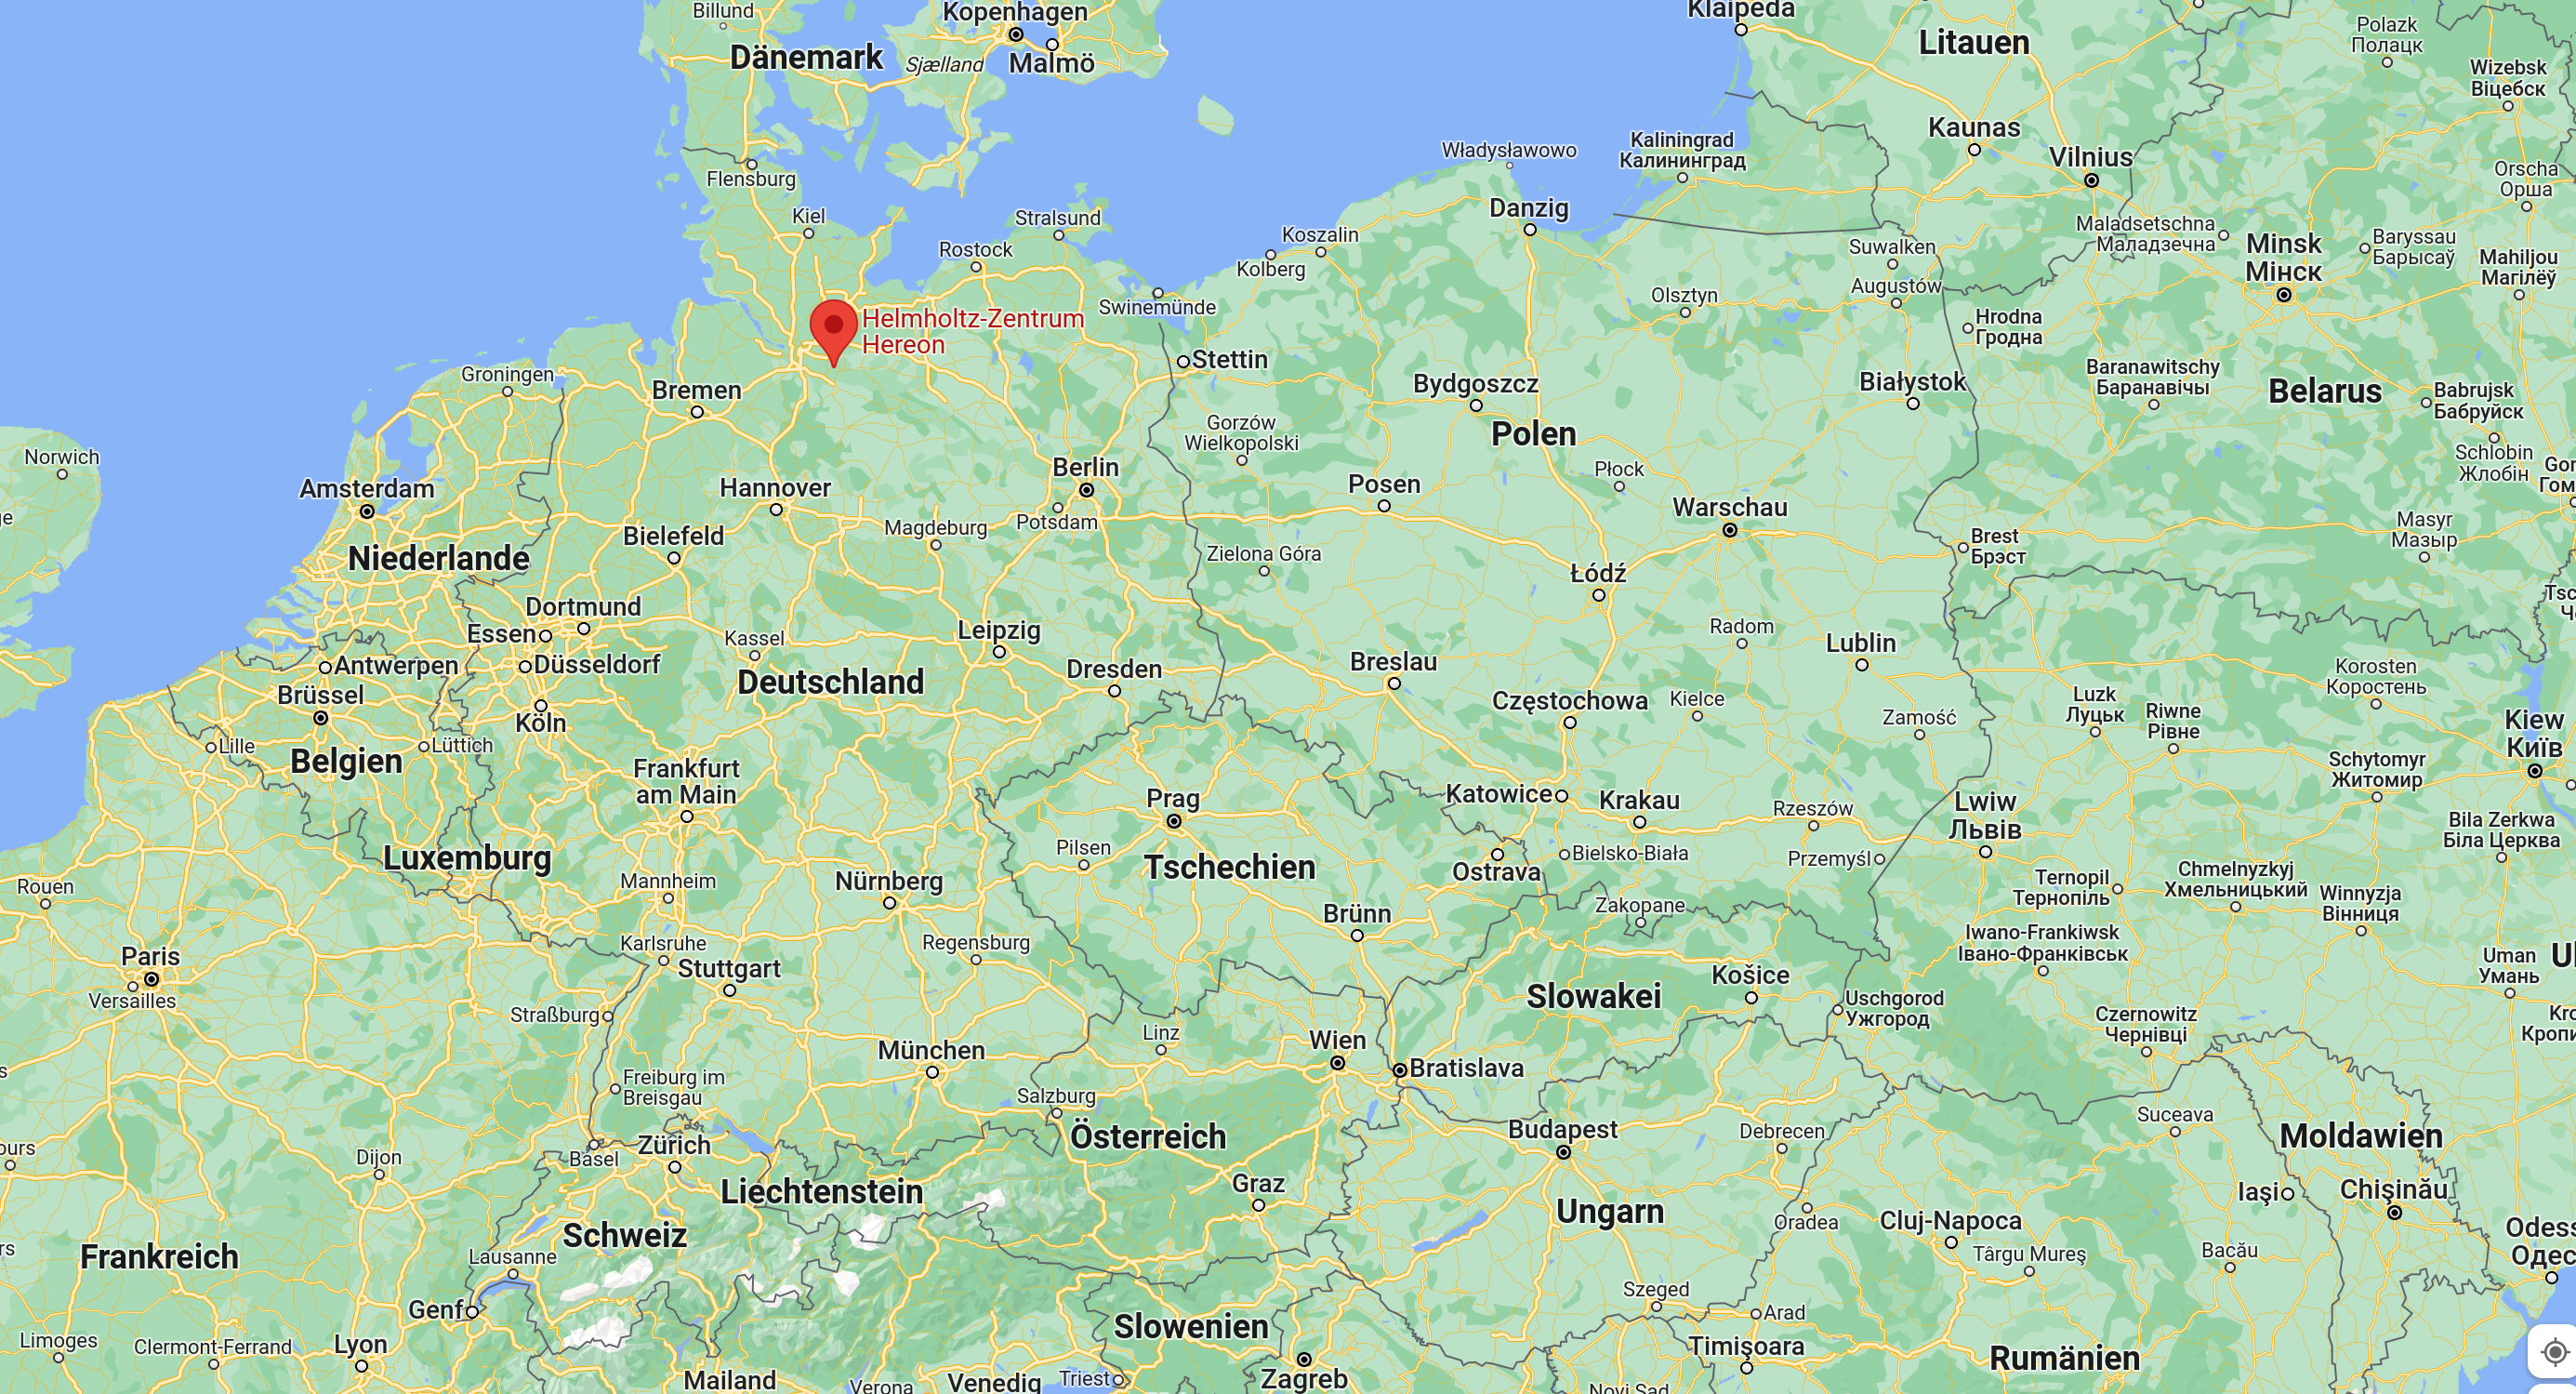
\includegraphics[height=0.7\textheight]{figures/hereon-map.png} \rotatebox{90}{\hyperlink{frm:author}{\beamerbutton{Back to author page}}} \\
Helmholtz Coastal Data Center (HCDC) - Helmholtz-Zentrum Hereon \\
Max-Planck-Straße 1 - DE - 21502 Geesthacht \\
\end{frame}

\end{document}